\chapter{Physiological and Mathematical Background}

The heart is one of the most important organs in the human body.
It is responsible for pumping blood around the arteries and veins of the human
body to all of the organs within.
The blood carries all of the oxygen, energy and other substances needed for the
body to continue to live to all parts of the body.
It also bears away all of the carbon dioxide and other waste products so that
they can be removed.

The heart does this via rhythmic and synchronised contractions.
The contractions are, in the healthy heart, initiated from one place and
synchronised via electrical signals conducted through the heart.
This conduction is aided by a number of specialised cell types.

\section{The Heart}

The heart's role is to pump blood around the body, driving the circulation of
the blood and everything contained within it.  It is one of the most important
organs in the body and any malfunction in its behaviour could be fatal in very
short order.  It begins beating in the early stages of pregnancy and continues
until death, hopefully many decades later.  It beats at an average rate of
around 70 beats per minute (bpm) for the adult male and 75 bpm for the adult
female.

The heart is not, as popular belief would have it, the seat of human emotion.
The functioning of the heart is modulated by such emotion however, slowing when
we are calm and increasing in rate quite dramatically when we are excited or
afraid.  Despite being influenced by the brain and our emotional states, the
heart drives itself, rather than having the pace-making initiated outside the
organ.

\subsection{Location of the Heart}

The human heart sits in the centre of the chest, the bulk of it extending into the
left-hand side of the chest cavity, inside a fibrous sac called the pericardium.
The actual location, orientation and size can vary quite significantly from
individual to individual~\cite{Oberman1967}.


\subsection{Gross Structure of the Heart}

The heart is mostly muscle.
This muscle is anchored to a collagenous `skeleton', known as the annulus
fibrosus located at the atrio-ventricular junction.
The muscle is different from the `smooth' skeletal muscle, in both structure
and behaviour~\cite{Katz2006}.

The human heart has four chambers; two atria and two ventricles.  The atria receive
the blood from the circulatory system and force it into the two ventricles,
which then contract and force this blood out and around the lungs and body.
These chambers are known as the left and right atria and the left and right
ventricles.  The left hand side of the heart in humans is much more developed
than the right.
This is due to their differing roles in circulating the blood.

The right and left atria are smaller than their respective ventricles and have
much thinner walls, because they need to develop much less pressure.  The right
atrium receives the blood from the circulatory system which is de-oxygenated,
and passes it on to the right ventricle.  The left atrium receives the highly
oxygenated blood from the lungs, and passes it onto the left ventricle.  The two
atria are separated by a thin muscle wall known as the intra-atrial septum.
This prevents the mixing of blood between the two atrial chambers.

The differences between the right and left ventricles are much more pronounced
than those between the right and left atria.  The right ventricle must merely
pump blood around the lungs and developing too high a pressure there could
actually damage the delicate structures.  By contrast the left ventricle must
develop enough pressure to drive blood around the whole body and as such it is
much more muscular.  The two ventricles are divided by the ventricular
septum.

As noted earlier, separating the atria and ventricles is the annulus fibrosus
or central fibrous body.
This is a dense layer of fibrous tissue.
In addition to providing an anchor for the muscle of the heart, it electrically
isolates the atria from the ventricles.
In the normal heart, the only electrical connection between the atria and the
ventricles is at the atrio-ventricular node.
This connects the right atrium to the specialist conduction system of the
ventricles.

\subsection{The Atria}

Examination of the human atria (or auricles, in older literature) is as old as studies
of the heart.
However, in recent years there has been a renewed interest in the
atria and their structures.
This has followed an increasing appreciation that the atria are not merely
reservoirs of venous blood, but have an active role to play in the function of
the heart~\cite{Ho2002a,Ho2002b,Ho2009,Platonov2007,Platonov2008a}.

Descriptions of the location of features use the `altitudinal' description, where
this is possible.
Altitudinal descriptions use the coordinates of the body, such that `right' is
the body's right hand side, not the right of the observer.
In this description, the atria are located to the right of the ventricles.
They can be slightly superior, too.
The right atrium is anterior and to the right, the left atrium more posterior and to
the left of the body.

The atria have a number of common features.
Both have a valve on the base, which is part of the central fibrous body.
In the right atrium, this is the tricuspid valve, in the left, the mitral valve.
These valves feed into the respective ventricles.

Both atria also have appendages, although the appendages differ in form.
The right atrial appendage is large, with a triangular shape and a wide base.
It is located anteriorly and superiorly on the right atrium.
By contrast, the left atrial appendage is smaller and more tubular in nature.
It is located posteriorly and superiorly compared to the left atrium.

\subsubsection{The Right Atrium}

The right atrium gathers in blood from the body, after it has cycled around the
organs.
The right atrium has a simpler topology than the left atrium.
At the top is an opening for the superior vena cava, and at the base there are
openings for the inferior vena cava and the tricuspid valve.

The right atrium is the location of many of the important sites of the
conduction system of the heart.
The sinus node, or sino-atrial node (SAN), is located on the right atrial wall,
close to the superior vena cava.
The SAN is the primary pacemaker for the heart in normal function.
It achieves this through specialised cells, known as nodal cells.
These cells are what are termed `auto-active' and are capable of spontaneously
exciting.

Running down the lateral wall is a muscle ridge, known as the crista terminalis,
or terminal crest.
The crista terminalis delineates the smooth and rough parts of the right atrial
wall.
This muscle ridge consists mostly of myocytes---cardiac muscle cells---arranged
longitudinally along the main axis of the ridge, and so forms a path of
preferential conduction.
In addition, these cells have a specialised electrophysiology~\cite{Feng1998}.

At the inferior end of the crista terminalis there is the atrio-ventricular
node (AVN).
This is another area of specialised nodal cells.
These cells are also auto-active, although with a slower natural frequency than
the SAN.
They therefore only take over in the case of SAN failure.
The AVN is the only point of electrical contact between the atrium and
ventricles in the normal heart.
As well as providing a link between the atria and ventricles this region acts
to limit the rate of stimulus which is passed on to the ventricles, protecting
them from excessive atrial pacing rates.

Branching from the crista terminalis and spreading around the muscle wall of the
right atrium are the pectinate muscles.
Like the crista terminalis, these bundles consist mostly of cells lying end to
end, forming pathways of preferential conduction.
The conformation of the pectinate muscles varies between individuals; some have
complex branching and interwoven patterns, whilst others have simpler and
relatively parallel bundles.

\subsubsection{The Atrial Septum}

The atrial septum divides the two atria.
Much of the septum is actually an in-folding of the right atrium.
The true septum is limited to the fossa ovalis and the muscle ring immediately
surrounding it.
The fossa ovalis is a valve which is important in fetal circulation, but is
closed in the normal adult.
The fossa ovalis is mostly fibrous in nature.
The muscle fibres run in a predominately circular direction around the fossa.

\subsubsection{The Left Atrium}

The left atrium gathers blood from the lungs.
The pulmonary veins tend to give the left atrium a more complex topology than
the right.
This complex topology can make the pulmonary veins a source of arrhythmic
activity.

Unlike the right atrium, the left atrium is not dominated by the appendage.
In the left atrium, the appendage is small and largely separate from the main
body of the atrium.
The endocardial surface of the appendage is covered in many fine muscle ridges.
Between these ridges, the walls of the atrium can be paper thin.

Conventionally the left atrium is depicted as having four openings for the
pulmonary veins.
Recent studies, reviewed in~\cite{Ho2009}, suggest considerably more variation
with approximately one third of hearts having merged veins on one or both sides.
In some cases, the single vein can actually link all the way to the lungs.
The pulmonary veins are surrounded by a sheath of tissue.
There is evidence that cells in the sheaths can have different electrophysiology
to normal atrial cells~\cite{Jones2008}.

The left atrial wall is relatively smooth.
However, it is not uniform in thickness or muscle architecture.
It instead has a complex and overlapping muscle structure.
This can look like layers, but there are no insulating fibrous sheets between
bundles.

\subsubsection{Inter-atrial Connections}

The atria are linked by muscle bundles.
These muscle bundles have cells mainly oriented end to end, which gives
preferential conduction along their axis.
The most well known of these is the Bachmann's bundle, which is located
anteriorly and superiorly between the two atria.

Common thought has it that the Bachmann's bundle is the principle electrical
connection between the atria in sinus rhythm.
However, recent studies (summarised in~\cite{Platonov2007,Platonov2008a}) have
found that in a significant fraction of the population, a secondary pathway
which is inferior and/or posterior is used instead.
In some subjects, a Bachmann's bundle cannot even be located.
There are a lack of studies performed on healthy subjects, however, so it is
unclear what occurs in the normal case.

\subsection{Cardiac Myocytes}

Myocytes, or muscle cells, comprise the vast bulk of cardiac tissue.
They both conduct electrical signals and contract to provide the force needed to
pump the blood around the body.
This is accomplished by a complex interplay of ionic
currents~\cite{Katz2006}.

\subsubsection{Myocyte Structure}

A typical human myocyte is from 50 to 150$\,\mu$m long, and has a radius
between 10 and 20$\,\mu$m.
They have a roughly cylindrical shape.
The cell is wrapped in an impermeable membrane, called the sarcolemma or plasma
membrane.
The membrane in many myocytes is invaginated at various points by series of
fine transverse tubules (T tubules) that carry action potentials deep into the
myocytes.

The cellular membrane contains a large number of specialised structures
responsible for allowing a regulated flow of ions into and out of the cell.
These structures include passive channels, active pumps and gated channels.
They are used to modulate the ionic composition of the intracellular
space and play a vital role in modulating the electrical activity of the cell.
Because it is impermeable a potential difference can build across the membrane
between the inside and outside of a cell.
This is the membrane potential.

Within the cells, much of the space is filled with what are called
myofibril-like units, long branching fibres about 1$\mu$m in diameter.
These fibres are divided up into sarcomeres, approximately 2$\mu$m long in the
resting myocyte, which is considered the basic contractile unit.
Mitochondria, which provide the ATP needed to provide energy for the
contractions, also occupy a significant fraction of the intracellular space.
Mitochondria are not actually a part of the body in the strictest sense and
have their own DNA -- they are symbiotic organisms that entered our own cells
at some unknown time in the past.
One other structure within the cells that is important to the electrical and
mechanical behaviour of the cells is a second tubule network, known as the
sarcoplasmic reticulum (SR) and the sarcotubular network.
The SR stores calcium in subsarcolemmal cisternae, which is released during the
membrane depolarisation.
The cisternae form structures known as dyads (or diads) with the T tubules.

\subsubsection{Ion Channels and Pumps}

The structures in the cellular membrane which permit ions to cross can
be roughly divided into channels and pumps.
Most channels and pumps are specific to one specific ion type.
Channels passively allow ions to flow with the concentration gradient, whilst
pumps actively move ions, regardless of the gradient~\cite{Hille2001}.

Channels and pumps are classified by the ion(s) they transport and how they are
controlled.
They are also classified on the direction of charge flow.
An inward current is one that would have the effect of a positive ion entering
the cell and could therefore also be caused by negatively charged ions exiting
the cell.
Inward currents act to increase the potential in the cell.
Conversely, outward currents are those that would have the effect of a positive
ion leaving the cell.
They are repolarizing currents as they act to decrease the membrane potential.

Inter-cardiac current flows through the gap junctions, which allow for large
current flows.
These are formed at the centre of membrane structures known as intercalated
disks.
The intercalated disks are concentrated at the ends of cells, although there are
some transverse connections.

Channels rely on an ionic gradient to drive flow through them.
Some channels have a constant conductance.
These are typically called background currents.
Channels with a conductance which depend on the instantaneous membrane potential
are known as voltage-gated channels.
Other channels can have their conductance modulated by the presence of a
hormone or chemical, such as the ATP sensitive potassium channel.
\begin{figure}
\begin{center}
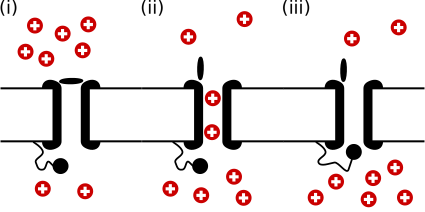
\includegraphics{figures/intro/activation_gate}
\end{center}
\caption[Time-Dependent Ion Channel]{
\label{fig:intro:heart:gated_ion}
A time dependant ion channel, represented by the black structure which bisects
the membrane (horizontal lines) for positive ions, shown as red circles.
The channel has an activation gate, the black lozenge on the top of the
membrane and an inactivation gate, the ball and chain on the underside of the
membrane.
In panel (i) the gate is not activated and shows a large concentration of ions
on the upper side.
In panel (ii), the gate activates and ions flow down the channel to the region
of lower concentration.
In panel (iii), the inactivation gate has moved to close the channel and no more
ions flow.
}
\end{figure}
Many gated channels are what are known as time-dependent channels.
These channels have structures over one or both ends which modulate the total
conductance to open (activate) or close (inactivate) the channel.
This is illustrated in figure~\ref{fig:intro:heart:gated_ion}.
The time course of this activation or inactivation is normally modulated by the
voltage, but can also be modulated by ion concentration or other mechanisms.
\begin{figure}
\begin{center}
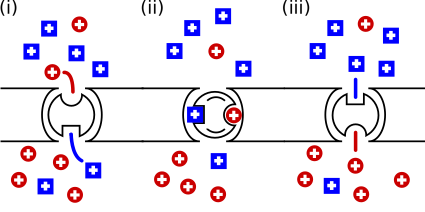
\includegraphics{figures/intro/ion_pump}
\end{center}
\caption[Ion Pump]{
\label{fig:intro:heart:ion_pump}
An ion pump (or more accurately, an ion exchanger), represented by the black
structure which bisects the membrane (horizontal lines) for two species of
positive ion, represented by red circles and blue squares.
The pump works against the concentration gradient.
In panel (i), the two ions bind to their respective sites on the pump.
In panel (ii), the pump changes its structure, drawing each ion through the
membrane.
In panel (iii), the pump releases the binding of the ions, letting them rejoin
the free ion populations.
}
\end{figure}
Pumps use energy to actively move ions against the gradient.
Complex molecules latch onto the ions on one side of the membrane and move them
through to the other side.
Many pumps are actually exchangers, which take in ions of one sort on one side
whilst transporting another type of ion the other way.

\subsubsection{Myocyte Electrical Action Potentials}

The evolution of the electrical state of the cell, from polarised to depolarised
and back again is termed the action potential (AP).
The shape and duration of
the action potential is mostly determined by the channels, carriers and pumps
across the cellular membrane, though the internal and external concentrations of
several ions and molecules can also have a significant effect.
There are three
principle ion species involved in the development of the action potential;
sodium ($\text{Na}^{\text{+}}$), potassium ($\text{K}^{\text{+}}$) and calcium
($\text{Ca}^{\text{2+}}$).
The third, calcium, is also important for contractile function.
Chlorine ($\text{Cl}^{\text{-}}$) is also of importance in some cells.

\begin{figure}
\begin{center}

\includegraphics{figures/intro/ap_profile}
\end{center}
\caption[Schematic AP Profile]{
\label{fig:intro:heart:ap}
A schematic AP profile.
Labelled are the five phases of the action potential.
Phase 0, the upstroke.
Phase 1, the end of the upstroke.
Phase 2, the plateau.
Phase 3, the repolarization.
Phase 4, the resting period.
}
\end{figure}

The action potential has 5 phases (figure~\ref{fig:intro:heart:ap}).
It begins with depolarization, phase 0.
During depolarisation, the current is carried principally by the fast inward
sodium current.
Phase 0 is also known as the upstroke of the action potential, and its slope is
important to the propagation of the action potential through cardiac tissue and
also the excitability of the myocyte as in individual cell.
Phase 0 is over almost instantaneously in healthy myocytes.

Phase 1 signifies the end of the upstroke, and is caused by the inactivation of
the sodium channels.
The small notch present in some cellular action potentials is caused by a
transient net outward current, carried principally by potassium.

Phase 2 is the plateau phase.  This relatively long phase ($>$100ms in some
myocytes) is due to the balance of slowly activating inward calcium currents and
the outward potassium currents.
The inward calcium current is principally carried by the L-type calcium channels
and the outward potassium current by a plethora of channels, classified by the
speed of activation or the substance which modulates them.

Phase 3 is the repolarization period.
The calcium channels have inactivated.
The potassium currents are still open, and the net efflux of positive charge
repolarizes the cell.

The final phase 4 is the period during which the cell is at the resting
potential.
In addition, for a short period of phase 4, the cell is in fact
impossible to excite above this resting potential due to the inactivations of
numerous channels.
This is called the refractory period.

Both the shape and the length of the action potential have physiological
importance.
Many pathological conditions have a significant impact upon both.
The action potential duration (APD) is often given as an \apd\ or
\apd[50], denoting the duration of the AP at 90\% or 50\% repolarization,
respectively.

The action potential upstroke (phase 0) is initiated when the potential difference across
the cellular membrane is raised above a particular level.
This is known as the threshold of excitation.
Stimuli which fall below this threshold won't elicit an excitation, whilst those
which cross it, will.
The threshold is influenced by a number of factors, but the fast sodium channel
is the most important determinant; when the fast sodium channel opens far
enough, the influx of sodium ions soon fully depolarizes the cell.

In normal cardiac tissue, the upstroke is initiated due to current flows between
cells that raise the potential of the cells around an active cell.
This happens in the extracellular medium, but also through the gap
junctions.
The sodium (and other) ions can flow through the non-specific channels formed by
the gap junctions.

\section{Mathematical Models of the Heart}

Cardiac tissue has been modelled mathematically for about fifty years.
While initial models were simple, there are now models of high sophistication
available.
These models are capable of reproducing both healthy and pathological behaviour
with some accuracy.

\subsection{Advantages of Mathematical Models}

Mathematical modelling offers an attractive alternative to experiments on
cardiac tissue.
This is particularly true when it comes to studies of human cardiac tissue.
However, there are advantages to models of cardiac tissue in all species.

One powerful advantage cardiac models offer is that of dissecting the root cause.
To express this another way, they aid in investigation of which particular
change is the most significant in a case such as a disease or genetic disorder.
In experiments on electrophysiology, the ability to modulate currents depends on
the existence of a drug to block (or open) the channel or even creating an
organism which doesn't express the gene, such as a `knock out mouse'.
In a computer model, this is as easy as removing an equation or tweaking a
parameter.
This can be used to suggest a drug treatment regime for patients.
Of course, such a suggestion will require clinical trials, but modelling can
eliminate non-starters.

Closely linked to the idea of examining the most significant change, cardiac
models can also allow people to `look within'.
This can be achieved on a number of scales.
Cellular models can report on the ionic concentrations, tissue models allow the
voltage distribution to be explored at any level, ECG models allow the
comparison of a known cardiac state and the resulting ECG.
This can, again, be used to suggest further therapies or diagnosis.

Cardiac models have a particular importance when it comes to human models.
Due to ethical considerations, the supply of human cardiac tissue is limited.
Most commonly it comes from posthumous donations of the heart or from biopsies
taken during cardiac surgery.
Both have obvious disadvantages.
In one case, the tissue is dead and thus not suitable for functional studies.
In the other, the biopsy itself may be from pathological tissue and is therefore a
poor guide to healthy function.
Gathering data from the functioning human heart requires surgical intervention,
which must necessarily be kept brief.
Models built from our understanding of how the mammalian heart functions and
the human electrophysiological data currently available therefore offer some of
our best insights into human cardiology.

Another benefit, which cannot be wholly ignored, is cost.
It is quite possible to perform many cardiac simulations on mid- to high- level
desktop PC, costing no more than \pounds 1000.
This includes modelling of cardiac tissues in three dimensions.
Conversely an electrophysiological laboratory can run to tens of thousands of
pounds and that does not include raw materials or animal subjects.

One common theme is the synergy that can emerge between experimental or clinical
work and mathematical modelling.
This can be exploited in work such as patient specific
modelling~\cite{Sermesant2006,Ramanathan2006}\ where a model is adapted to the pathology of a
specific individual.
Models can also be used to suggest hypothesis, such as the role of fibroblasts
in cardiac function and again~\cite{Kohl2005}, which can then be investigated
further in an experimental setting.
To draw on an example from this thesis, the \ii{ANION} case study, they can
also be used to look beyond what is currently possible to examine
experimentally, due to a lack of available drugs and suggest whether developing
such drugs might be worthwhile.

\subsection{Categorising Myocyte Models}

Cellular models tend to be classified in two ways.
The first differentiator is the level of detail employed.
The second is which cellular processes are modelled.

Biophysically detailed models are complex.
They consider the interactions of several different currents, and potentially
intra- and extracellular ion concentrations, reservoirs as well as other
details.
The second type are simplified, phenomenological, models.
These do not consider individual ion concentrations but instead just reproduce
one desired factor, typically the action potential profile.

Models, whether biophysically detailed or not, can concern themselves with the
cellular electrophysiology, the mechanical contractions or both.
This thesis concerns itself just with electrophysiological models.
Models of the mechanics are not considered and are not treated in this
description of mathematical modelling.

\subsection{A Brief History of Cardiac Myocyte Modeling}

The first model of cardiac electrophysiology was published by
Noble~\cite{Noble1962}, and modelled Purkinje fibre (A specialised part of the
ventricular conduction system) action potentials.
Shortly thereafter, various refinements were published, as further experimental
data became available.
This was eventually followed by the Beeler--Reuter~\cite{Beeler1977}\ model of
the guinea pig ventricular myocyte.

The Luo--Rudy guinea pig ventricular myocyte model was first published in
1991~\cite{Luo1991} and was then sub-sequentially majorly revised and
republished in 1994~\cite{Luo1994}.
The first Luo-Rudy model was based on the Beeler--Reuter model, though with updated channel behaviours
and more complex potassium channels.
The second Luo-Rudy model was the first of the `second generation' models,
with fluctuations in all ion concentrations, and a much more detailed series of
equations for calcium handling.

In 1998, the Courtemanche--Ramirez--Natel\cite{CRN98}\ (CRN) model and the
Nygren~\cite{Nygren1998}\ model were published.
These were both models of the human atrium.
They were also both second generation models, with detailed calcium handling.
Also in 1998 Fenton and Karma published their phenomenological
Fenton--Karma~\cite{Fenton1998}\ model, which used just three channels to
reproduce the shape of the ventricular action potential.

\subsection{Mathematical Models of Myocytes}

Mathematical models of cardiac myocytes are built from a few simple assumptions
and considerations.
These concern the behaviour of the cellular membrane and ion channels.
The important ones are detailed here.

\subsubsection{The Nernst Equilibrium Potential}

The Nernst equation is an important equation in electrophysiology~\cite{Fall2002}.
It describes how the difference in ion concentrations on two sides of a
semi-permeable barrier can result in a potential difference across the barrier.
Any voltage dependant factor of a current of an ion, S, includes a reversal
potential, $V_{S}$, equal to the Nernst potential.
At the reversal potential, the current falls to 0.
When equilibrium is reached the potential difference, $V_{S}$, across the
membrane is given by
\begin{equation}
V_{S} = \frac{RT}{zF}ln\left( \frac{[S]_{e}}{[S]_{i}} \right) 
\end{equation} 
where subscripts $i$ and $e$ denote internal and external concentrations of S,
$R$ is the universal gas constant, $T$ is the absolute temperature, $F$ is
Faraday's constant and $z$ the charge of the ion $S$.

The Nernst potential applies only to a single ion concentration.
Since many ion channels are ion channel specific, the Nernst potential can still
be used to calculate the driving potential.

\subsubsection{Electric Circuit Model}

\begin{figure}
\begin{center}

\includegraphics{figures/intro/electrical_circuit_cell}
\end{center}
\caption[Electrical Circuit Model Of The Cell]{
\label{fig:intro:math:circuit}
Electrical circuit representation of the cell.
The cell membrane is represented by a capacitance, $\text{C}_{\text{m}}$.
There are three currents, represented by the conductances $\text{g}_{\text{K}}$,
$\text{g}_{\text{Ca}}$ and $\text{g}_{\text{Na}}$.
The current through the resistances is driven by the three Nernst potentials,
$\text{E}_{\text{K}}$, 
$\text{E}_{\text{Ca}}$ and $\text{E}_{\text{Na}}$.
}
\end{figure}

The electrical circuit model of the cell membrane underpins much of the work in
modelling the behaviour of cardiac myocytes.
It is however a very simple concept.
Since the membrane separates charges, it may be considered as a capacitor, as
shown in figure~\ref{fig:intro:math:circuit}.
Since there is no net buildup of
charge on either side of the membrane, any ionic current, \ii{ion}, must be
countered by a capacitive current, and so
\begin{equation}
C_{m}\frac{dV_{m}}{dt} + \ii{ion} = 0
\label{eqn:intro:math:basic}
\end{equation}
where $V_{m}$ is the membrane voltage, and is defined as the difference between
the internal potential, $u_{i}$ and the external potential, $u_{e}$ or
\begin{equation}
V_{m} = u_{i} - u_{e}
\label{eqn:intro:math:vm}
\end{equation}
When multiple currents are considered, the total inward and outward currents are
summed.
The difficulty comes in determining the form of \ii{ion}, which varies widely
depending on the nature of the channel or pump in question.


\subsubsection{The Hodgkin-Huxley Equations}

Many mathematical models of cardiac myocytes feature one or more
`Hodgkin--Huxley' channels.
Hodgkin and Huxley developed them in a now classic series of papers concerning
the current flow through the membrane of the squid giant
axon~\cite{Hodgkin1952,Keener1998}.
They characterise the current flow with elegance and surprising accuracy.
It is important to note that the Hodgkin--Huxley equations consider the bulk
behaviour of the many thousands of individual channel structures distributed
across the membrane, not the behaviour of one single channel.

Hodgkin and Huxley started with a very simple assumption.
The current flow through a channel on the membrane, $I_{S}$ is given by
\begin{equation}
I_{S} = g_{S}\left(V-V_{S}\right)
\label{eqn:intro:math:hh1}
\end{equation}
where $g_{S}$ is the channel conductance, $V$ the membrane potential and $V_{S}$
the Nernst potential for the ion $S$.
Equation (\ref{eqn:intro:math:hh1}) assumes that the channel is selective for
one ion species S, and that the current is a simple linear function of the
voltage across the membrane.

With this underlying assumption, Hodgkin and Huxley set out to accurately map
the behaviour of the current with regards time and voltage.
The following section explains the description for the sodium current, \ii{Na}.
From the form of the sodium channel under voltage clamp conditions, it is
reasonable to expect $g_{Na}$ obeys a differential equation of the form
\begin{equation}
\frac{dg_{Na}}{dt} = f\left(v,t\right)
\label{eqn:intro:math:hh2}
\end{equation}
where $v=V-V_{Na}$.
However, the form of $g_{Na}$ is complex.
While remaining at the same voltage, the conductance at first increases and then
tails off.
It appeared that there were two processes at work, one that turned the current
on, and one that turned it off.
Hodgkin and Huxley realised that it would be easier to write $g_{Na}$ as a
function of two different variables.
One which corresponded to the turning on and one to the turning off of the
channel.
This leads to there being an activation variable, called $m$, an inactivation
variable, called $h$ and that the current would be some linear combination of the
two, multiplied by a constant conductance factor $\bar{g}_{Na}$.
The two variables $m$ and $h$ would both satisfy a differential equation such as
\begin{equation}
\frac{dm}{dt}=\alpha_{m}\left(v\right)\left(1-m\right) -
\beta_{m}\left(v\right)m
\label{eqn:intro:math:dmdt}
\end{equation}
where $\alpha_{m}$ and $\beta_{m}$ are functions of $v\,\left(=V-V_{Na}\right)$.
As $m$ is an activation, $\alpha_{m}$ and $\beta_{m}$ are such that $m$ is
initially small but increases with the potential allowing current to flow within
the channel.
As $h$ is an inactivation, $\alpha_{h}$ and $\beta_{h}$ give an initially high
value of $h$ that then decays, inactivating the channel.

The form proposed for $g_{Na}$ by Hodgkin and Huxley was
\begin{equation}
g_{Na}=\bar{g}_{Na}m^{3}h
\label{eqn:intro:math:gna}
\end{equation}
where all symbols are as defined previously.
The decision to raise $m$ to the third power was based on the rate of increase
observed in voltage clamp experiments.
It is interesting to note that when the structure of \ii{Na}\ was examined in
detail, it was discovered that the channel has three structures which open to
allow current to flow.
A second type of structure, the `ball and chain', then acts to close the channel.

Many different channels are modelled as Hodgkin--Huxley channels.
Different channels have different activation and inactivation variables.
These variables are modulated by different $\alpha$ and $\beta$ equations.

\subsubsection{Markov Chain Descriptions Of Ion Channels}

Markov chain models of ion channels~\cite{Balser1990,Clancy1999,Silva2005}\
emerged when more detailed information on ion channels became
available.
This included single channel recordings rather than whole cell recordings.
In such conditions, as well as in certain pathological states, the
Hodgkin--Huxley descriptions of the cells broke down.

In a Markov chain model, instead of having one or more activations or
inactivations, the channel has a number of states.
Common states can include open, inactive and closed.
A channel can have more than one state of each sort.
Transitions are only allowed between certain states and each transition has a,
usually time or voltage dependent, probability.
Channels only allow current to flow whilst in an open state.

Markov chain models can be highly complex and contain many states.
They can be utilised in a variety of ways.
One Markov chain can represent the behaviour of all the individual channels on
the cell.
In this case, the total current flowing in the channel will be proportional to
the fraction of open states.
Cells can also have multiple Markov chains to represent the flow through a
channel, each with its own proportions of state occupancy.
They also open the possibility of using stochastic simulation techniques where
the transition between states is controlled by random chance.

\subsection{Selected Myocyte Models}

There are many myocyte models of varying complexity and
accuracy.
There are relatively few models of atrial myocytes for human tissue.
A brief description of the foremost two are given here, as well as a description
of one of the most adaptable phenomenological models.

\subsubsection{The Courtemanche--Rameriz--Nattel Model}
\label{sec:intro:math:crn}

The Courtemanche--Rameriz--Nattel (CRN) model~\cite{CRN98}\ is a biophysically
detailed second generation model of the human atrial myocyte.
It was based on the Luo-Rudy~\cite{Luo1994}\ model of the guinea pig ventricular
myocyte.
The currents were then modified based on data from human and animal atrial
myocytes.
It produces action potentials with a spike and dome morphology.

The CRN model tracks 21 state variables.
Most of these are gating parameters for the many ion channels, but the model
also tracks the internal concentration of potassium, sodium and calcium ions.
The external concentrations of ions are assumed constant.
There are also state parameters representing the calcium stored in internal
structures, such as the sarcoplasmic reticulum.
\begin{align}
\label{eqn:intro:math:crn}
\ii{ion} = \ii{Na} + \ii{K1} + \ii{to} + \ii{Kur} + \ii{Kr} + \ii{Ks} + 
\ii{Ca,L} \nonumber \\
+ \ii{b,Na} + \ii{b,Ca} + \ii{NaK} + \ii{NaCa} + \ii{p,Ca}
\end{align}
The CRN has 12 transmembrane currents and pumps which contribute to \ii{ion},
equation~(\ref{eqn:intro:math:crn}), and 4 currents and
pumps which just interact with the internal calcium stores.
The external currents are \ii{Na}, the fast sodium current, \ii{K1}, the inward
rectifier potassium current, \ii{to}, the transient outward current, \ii{Kur}, the
ultra-rapid delayed rectifier current, \ii{Kr}, the rapid delayed rectifier
current, \ii{Ks}, the slow delayed rectifier current, \ii{Ca,L}, the L-type
calcium current, \ii{b,Na}, the sodium background current and \ii{b,Ca}, the
calcium background current.
All the currents are time-dependent and voltage, except for the background currents which
have constant conductance and \ii{K1}, which is just voltage-dependent.
There are also three pumps; \ii{NaK}, the sodium--potassium exchanger,
\ii{NaCa}, the sodium--calcium exchanger and \ii{p,Ca}, the calcium pump.

As a biophysically detailed model, the CRN model is suitable for a variety of
modelling tasks.
The number of currents make it an attractive option for modelling drugs or
genetic mutations.
It can be expensive to solve for large numbers of cells, however.

\subsubsection{The Nygren Model}

The Nygren model~\cite{Nygren1998}\ is a biophysically detailed second
generation model of the human atrial myocyte.
It was based on the Linblad~\cite{Lindblad1996} model of the rabbit atrium.
The equations were then modified using human data, mostly gathered from the
atrial appendages.
It produces triangular action potentials.

The Nygren model tracks 29 state variables.
Most of these are gating parameters.
They model also tracks concentrations of ions, both internally and in
extracellular cleft spaces, to represent local ion fluctuations.
Like the CRN model, there are also variables to represent internal calcium
handling.
\begin{align}
\label{eqn:intro:math:nygren}
\ii{ion} = \ii{Na} + \ii{K1} + \ii{to} + \ii{Kur} + \ii{Kr} + \ii{Ks} + 
\ii{Ca,L} + \nonumber \\
\ii{b,Na} + \ii{b,Ca} + \ii{NaK} + \ii{NaCa} + \ii{p,Ca}
\end{align}
The Nygren model has 12 transmembrane currents and pumps which contribute to \ii{ion},
equation~(\ref{eqn:intro:math:nygren}), and 4 currents and
pumps which just interact with the internal calcium stores.
The external currents are: \ii{Na}, the fast sodium current, \ii{K1}, the inward
rectifier potassium current, \ii{to}, the transient outward current, \ii{Kur}, the
ultra-rapid delayed rectifier current, \ii{Kr}, the rapid delayed rectifier
current, \ii{Ks}, the slow delayed rectifier current, \ii{Ca,L}, the L-type
calcium current, \ii{b,Na}, the sodium background current and \ii{b,Ca}, the
calcium background current.
All the currents are time- and voltage-dependent, except for the background
currents which have constant coductance and \ii{K1}, which is voltage-dependent.
There are also three pumps; \ii{NaK}, the sodium--potassium exchanger,
\ii{NaCa}, the sodium--calcium exchanger and \ii{p,Ca}, the calcium pump.

The Nygren model has more involved mathematics and requires more storage than
the CRN model, making it less attractive for large-scale simulation.
It is also interesting to note that the two models have very different
AP morphologies, the reasons for which have been the subject of some
research~\cite{Nygren2001,Syed2005,Cherry2008}.

\subsubsection{The Fenton--Karma Model}
\label{sec:intro:math:fk}

The Fenton--Karma (FK) model is a
phenomenological, minimal variable, model of the ventricular action
potential.
The goal of the FK model is to accurately reproduce the AP profile and
restitution properties of myocytes as well as short-term memory effects.
The original FK model has 3 variables, a fourth was added
recently~\cite{Fenton1998,Bueno-Orovio2008}.

The FK model tracks 4 state variables.
These have no true physiological analogues, but certain correlations can be
drawn.
\begin{equation}
\label{eqn:intro:math:fko}
\ii{ion} = \ii{fi} + \ii{si} + \ii{so}
\end{equation}
The FK model has 3 transmembrane currents which contribute to \ii{ion},
equation~(\ref{eqn:intro:math:fko}).
The fast inward current, \ii{fi}, is roughly analogous to the fast sodium
current in more detailed models, the slow inward current, \ii{si}, fulfils a
similar role to the L-type calcium current and the slow outward current, \ii{si},
is analogous to the potassium rectifier currents.
The behaviour of the currents is generally controlled by step functions based
on the state variables.

The FK model is not biophysically detailed.
This makes it very fast to solve, making it attractive for large tissue
simulations.
The drawback of this is that incorporating complex hormonal or drug interactions
is difficult.
The model is highly modifiable, with parameter sets that can reproduce a variety
of AP morphologies and restitution behaviours, including one for atrial myocyte
APs~\cite{Weber2008}.

\subsection{Models of Action Potential Propagation}

Single myocyte models are important, and can tell us much about the heart in
disease and health.
The heart is not made up of isolated myocytes however.
Whilst current computational power does not allow myocytes to be modelled on an
individual cellular basis for the whole heart, continuum models of propagation
have been developed.
These are summed up in the bidomain equations, and their simplification, the
monodomain equations.

\subsubsection{The Bidomain Equation}

The bidomain equation comes out of basic electromagnetic theory and several
assumptions about the nature of cardiac tissue~\cite{Tung1978,Geselowitz1983}.
\begin{enumerate}
    \item The cardiac tissue contains two continuous, simply connected domains,
    the intracellular and extracellular domains separated by the cell membrane.
    There is no detailed consideration of the fine points of geometry.
    \item The intra- and extracellular domains overlap and fill all of the cardiac muscle. Each point lies in both domains.
    \item Charge does not accumulate.
\end{enumerate}

The derivation, starting from Maxwell's Equations, is not that difficult to work
through.
\begin{equation}
\label{eqn:intro:math:maxwell}
\nabla x \mathbf{E} + \mathbf{\dot{B}} = 0
\end{equation}
Treating the situation as quasi-static with no rapid changes of field, $\mathbf{\dot{B}} = 0$, and so
\begin{equation}
\label{eqn:intro:math:maxwellqs}
\nabla x \mathbf{E} = 0
\end{equation}
In this situation, the electrical field, $\mathbf{E}$, can be written as the
divergence of some scalar field, $u$:
\begin{equation}
\label{eqn:intro:math:electricfield}
\mathbf{E} = - \nabla u
\end{equation}
The current which flows in the tissue, $\mathbf{J}$, is then given by the simple
relationship
\begin{equation}
\label{eqn:intro:math:current}
\mathbf{J} = \mathbf{M} \mathbf{E}
\end{equation}
where $\mathbf{M}$ is a tensor of the conductivities in the tissue.
Substituting in (\ref{eqn:intro:math:electricfield}) and using the subscripts
$i$ and $e$ to represent the intra- and extracellular domains, respectively,
expressions for the current flow in each domain are
\begin{subequations}
\label{eqn:intro:math:currentsubs}
\begin{align}
\mathbf{J}_i &=& - \mathbf{M}_i \nabla u_i
\label{eqn:intro:math:currenti}\\
\mathbf{J}_e &=& - \mathbf{M}_e \nabla u_e
\label{eqn:intro:math:currente}
\end{align}
\end{subequations}
Since no charge accumulates (our third assumption), the amount of current
entering a small volume, $\partial V$, must equal the amount of current leaving
the small volume
\begin{equation}
\label{eqn:intro:math:currentvolumeinteg}
\int_{\partial V} \left(\mathbf{J}_i + \mathbf{J}_e\right) \cdot d\mathbf{S} = 0
\end{equation}
The volume $V$ may be arbitrarily chosen and so using the divergence theorem
\begin{equation}
\label{eqn:intro:math:currentdiv}
\nabla \cdot \left(\mathbf{J}_i + \mathbf{J}_e\right) = 0
\end{equation}
Substituting in the equations (\ref{eqn:intro:math:currenti}) and
(\ref{eqn:intro:math:currente}) we obtain
\begin{equation}
\label{eqn:intro:math:currentdivsubst}
\nabla \cdot \left(- \mathbf{M}_i \nabla u_i \right) + \nabla \cdot \left(-\mathbf{M}_e \nabla u_e \right) = 0
\end{equation}
Any current which flows between the two domains must cross the cell membrane, so
\begin{equation}
\label{eqn:intro:math:currentdivim}
- \nabla \cdot \left(- \mathbf{M}_i \nabla u_i \right) = \nabla \cdot \left(-\mathbf{M}_e \nabla u_e \right) = I_m
\end{equation}
where $I_m$ is the transmembrane current.
There is already an expression for $I_m$, given by (\ref{eqn:intro:math:basic}).
This expression is per unit area of the cell surface, whereas we now want current per unit volume.
We therefore introduce $\chi$, the ratio of the cell surface area to the cell volume and so
\begin{equation}
\label{eqn:intro:math:im}
I_m = \chi \left(C_{m}\frac{dV_{m}}{dt} + I_{ion}\right)
\end{equation}

Combining (\ref{eqn:intro:math:currentdivsubst}),
(\ref{eqn:intro:math:currentdivim}) and (\ref{eqn:intro:math:im}) produces
\begin{subequations}
\label{eqn:intro:math:bidom3}
\begin{align}
\nabla\cdot\left(\left(M_{e}\right)\nabla u_{e}\right) + \nabla\cdot\left(M_{i}\nabla u_{i}\right) &=& 0
\label{eqn:intro:math:bidom31}\\
\nabla\cdot\left(M_{i}\nabla u_{i}\right) &=& \chi \left(C_{m}\frac{dV_{m}}{dt} + I_{ion}\right)
\label{eqn:intro:math:bidom32}
\end{align}
\end{subequations}
Which is two equations in three unknowns.  However previously
(\ref{eqn:intro:math:vm}) defined $u_i = V + u_e$ and so substituting and
re-arranging, the bidomain equations are obtained
\begin{subequations}
\label{eqn:intro:math:bidom}
\begin{align}
\nabla\cdot\left(\left(\mathbf{M}_{i}+\mathbf{M}_{e}\right)\nabla u_{e}\right) + \nabla\cdot\left( \mathbf{M}_{i}\nabla V_{m}\right) &=& 0
\label{eqn:intro:math:bidom1}\\
\nabla\cdot\left(\mathbf{M}_{i}\nabla V_{m}\right) + \nabla\cdot\left(\mathbf{M}_{i}\nabla u_{e}\right) &=& \chi \left(C_{m}\frac{dV_{m}}{dt} + I_{ion}\right)
\label{eqn:intro:math:bidom2}
\end{align}
\end{subequations}
where all symbols are as defined previously.
The bidomain equations are a coupled set of a parabolic and elliptic differential equation.

Boundary conditions for the bidomain equations vary, though the most common ones are described here.
First, no intracellular fluxes leave the heart.
Second, the body is assumed to be a passive conductor that is isolated at the outer surface.
The body potential at the surface of the heart is the extra-cellular potential at the surface of the heart.

\subsubsection{The Monodomain Equation}
\label{sec:intro:math:mono}

While the bidomain equations represent a good tool for modelling some of the complexities of cardiac conduction, they are very demanding to solve, necessitating finding the solution to coupled parabolic and elliptic differential equation sets.
The monodomain equation is the result of one simplifying assumption made to the bidomain equations.
For the monodomain equation, we assume that the anisotropy ratio, $\lambda$, is the same for the intra- and extra-cellular fluids at all points.
\begin{equation}
\mathbf{M}_{i} = {\lambda}\mathbf{M}_{e}
\label{eqn:intro:math:mratio}
\end{equation}
This assumption is not a very physiological one, but the simplification it
allows is significant and so it is quite commonly used.

Substituting (\ref{eqn:intro:math:mratio}) into (\ref{eqn:intro:math:bidom1})
and (\ref{eqn:intro:math:bidom2}) and rearranging reduces the pair of equations
to one single equation for the membrane potential
\begin{equation}
\frac{\lambda}{1+\lambda}\nabla\cdot\left(\mathbf{M}_{i}\nabla V_{m}\right) = \chi \left( C_{m}\frac{dV_{m}}{dt} + I_{ion}\right)
\label{eqn:intro:math:mono}
\end{equation}
Typically, the factor of ${\lambda}/\left({1+\lambda}\right)$ is folded into
$M_{i}$, along with $\chi$ and the membrane capacitance $C_m$ to give the diffusion tensor $D$.
In 1D, this is the cable equation.
The values of the components of the tensors $M_{i}$ or $D$ may be determined experimentally, or from a comparison of conduction in real and virtual tissue samples.

\subsection{Numerical Techniques}

There exist a wealth of techniques for solving the ordinary differential
equations (ODEs) and partial differential equations (PDEs) involved in
mathematical models~\cite{Sundnes2006}.
These techniques vary in complexity and accuracy.
The correct choice of technique depends on a number of factors including the
`stiffness' of the equations, the desired accuracy and others.

\subsubsection{The Forward Euler Method}

The forward Euler method~\cite{Birkhoff1989}\ is perhaps the simplest numerical
integration technique.
It requires a relatively small (time) step between integration points.
It is never--the--less quite suitable to use in simulations of the electrical
activity of the heart.
A typical set of ODEs representing the electrical activity of a myocyte are very
`stiff', which is to say they can be numerically unstable if the step size is
too large, and so more sophisticated methods can also require a very small
timestep.

The forward Euler method works as follows.
If we have a function, $f(t, u)$, for which we know the initial
values, $(t_0, u_0)$, then by assuming the rate of change of $f$ remains constant
over some small interval, $h$, we can integrate the equation as follows
\begin{subequations}
\label{eqn:intro:euler}
\begin{align}
t_{n+1} = & t_n + h \label{eqn:intro:euler:t} \\
u_{n+1} = & u_n + hf(t_n, u_n) \label{eqn:intro:euler:x}
\end{align}
\end{subequations}
As long as the interval is small enough the sequence $u_1,u_2,\cdots,u_n$
should be a good approximation of the time evolution of $u$.
If we have more than one value on the right hand side of the equation ($u =
u^{(1)}, u^{(2)}, \cdots, u^{(n)}$) then all values of the right hand side are
assumed constant for each step of the integration.
In cardiac systems, $h$ is typically \ms{0.02}\ or smaller.

\subsubsection{The Finite Difference Method}

The finite difference method~\cite{Morton2005} is a way of calculating the
solution to a spatially extended problem.
Such problems include PDEs such as the bidomain (\ref{eqn:intro:math:bidom}) and
monodomain (\ref{eqn:intro:math:mono}) equations.
The general form of such equations in the variable $u(t, u)$ is
\begin{equation}
\label{eqn:intro:fd:partial}
\frac{\partial u}{\partial t} = \frac{\partial}{\partial x} \left( b(t, x)
\frac{\partial u}{\partial x} \right) + c(t, x)u + d(t, x) + e(t, u)
\end{equation}
Where $t$ is the time, $x$ is the spatial variable and $b$, $c$, $d$ and $e$ are
known functions.
The function $e$ will quite often be \ii{ion}\ for a particular cell.

In the finite difference method, the problem space---the cardiac tissue, in this
thesis---is divided up into a number of nodes.
The spacing between each node is $\Delta x$ in the x direction (and in higher
dimensions,  $\Delta y$ in the y direction and so on).
To advance the solution in time, the forward Euler method
(\ref{eqn:intro:euler}) can be used.
To approximate the differential in space, the centred second difference can be
used.
For the node at $x_i$ at time $t_n$ it is:
\begin{equation}
\label{eqn:intro:fd:secondcentral}
\frac{\partial^2 u}{\partial x^2}\left(x_i, t_n\right) \approx \frac{u(x_{i+1},t_n) - 2u(x_{i},t_n) + u(x_{i-1},t_n) }{\left(\Delta x\right)^2}
\end{equation}
where $i$ is the index of the node, and $n$ the index of the instant of time.
The space centered first difference (needed when conduction anisotropy is to
be taken into account) is:
\begin{equation}
\label{eqn:intro:fd:firstcentral}
\frac{\partial u}{\partial x}\left(x_i, t_n\right) \approx \frac{u(x_{i+1},t_n) - u(x_{i-1},t_n) }{2\left(\Delta x\right)}
\end{equation}

The most common boundary conditions we want to apply are Neumann, `no flux',
boundary conditions where the differential of $u$ with respect to $x$ is set to
zero at the edges of the tissue.
At the edge of the tissue, the approximation for the space differential
(\ref{eqn:intro:fd:secondcentral}) becomes:
\begin{equation}
\label{eqn:intro:fd:secondcentralboundary}
\frac{\partial^2 u}{\partial x^2}\left(x_i, t_n\right) \approx \frac{2\left((u(x_{i-1},t_n) - u(x_{i},t_n) \right)  }{\left(\Delta x\right)^2}
\end{equation}
if the node at $x_{i+1}$ would be `outside' the tissue.
The approximation if the converse is true ($x_{i-1}$ is outside) replaces
$x_{i-1}$ with $x_{i+1}$.
The one dimensional approximation becomes:
\begin{equation}
\label{eqn:intro:fd:firstcentralboundary}
\frac{\partial u}{\partial x}\left(x_i, t_n\right) \approx \frac{u(x_{i},t_n) - u(x_{i-1},t_n) }{\left(\Delta x\right)}
\end{equation}
again, for if the node $x_{i+1}$ is outside.
\begin{figure}
\begin{center}
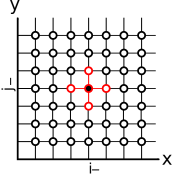
\includegraphics{figures/intro/stencil}
\end{center}
\caption[5--node Stencil for the Finite Difference Method]{
\label{fig:intro:math:stencil}
Representation of the finite difference method in two dimensions.
The stencil of the central node (solid black) is indicated in red.
}
\end{figure}
In higher orders, (\ref{eqn:intro:fd:secondcentral}) and
(\ref{eqn:intro:fd:firstcentral}) are applied along each direction.
The nodes used in the calculation of the value $u_x$ are known as the stencil.
The typical 5--node stencil used for solving (\ref{eqn:intro:fd:partial}) and
hence (\ref{eqn:intro:math:bidom}) or (\ref{eqn:intro:math:mono}) is illustrated
in figure~\ref{fig:intro:math:stencil}.
Other schemes can use different stencils.


\subsubsection{The Rush--Larsen Technique}

The Rush--Larsen technique~\cite{RL78}\ is a specialised way of solving
equations such as (\ref{eqn:intro:math:dmdt}) for the gating parameters.
Since $\alpha_m$ and $\beta_m$ are dependent only on the voltage, not on time, a
solution to (\ref{eqn:intro:math:dmdt})~\cite{Hodgkin1952} is:
\begin{equation}
\label{eqn:intro:math:dmdtsoln}
m = m_{\inf} - \left(m_{\inf} - m_0\right)\exp\left(-\frac{t}{\tau_m}\right)
\end{equation}
where
\begin{equation}
\label{eqn:intro:math:infm}
m_{\inf} = \frac{\alpha_{m}}{\alpha_{m} + \beta_{m}}
\end{equation}
and
\begin{equation}
\label{eqn:intro:math:taum}
\tau_m = \frac{1}{\alpha_{m} + \beta_{m}}
\end{equation}
where $m_0$ is the initial value of $m$.

Rush and Larsen realised that over a sufficiently small time interval, $\Delta t$,
the parameters $\alpha_m$ and $\beta_m$ could be considered constant.
Taking $m_0$ to be the value of $m(t)$ at time $t$, (\ref{eqn:intro:math:dmdtsoln})
could be used to calculate the next value of $m$, $m(t + \Delta t)$ as:
\begin{equation}
\label{eqn:intro:math:dmdtsolnrl}
m(t+ \Delta t) = m_{\inf} - \left(m_{\inf} - m(t)\right)\exp\left(-\frac{\Delta t}{\tau_m}\right)
\end{equation}
Using (\ref{eqn:intro:math:dmdtsolnrl}) is more accurate than the forward Euler
method (\ref{eqn:intro:euler}), since it depends only on the value of the
membrane potential, not the derivative of $m$.

\subsection{Limitations of Modelling}

Despite the inherent advantages of modelling, it does have disadvantages one
must be aware of as well.
Some of these are intrinsic to models, and others emerge from choices made.
Knowing the weaknesses of modelling can improve the conclusions drawn from
modelling.

One limitation of modelling is that often a choice must be made.
Phenomenological models offer very fast solution times, but do so by sacrificing
physiological detail.
Biophysically detailed models can offer more insight, but can be very slow to
solve, especially for tissue simulations.

The most obvious limitation of modelling is that a model can only ever be as
good as the assumptions and experimental data which are the input.
A model based on incomplete information or inaccurate assumptions is unlikely to
produce acceptable results.
Worse, it can lead to likely looking but erroneous results.

There is also the danger of extrapolation.
This can be particularly true for human models, which are often based on limited
data and supplemented by information from different animal tissues.
One clear example of this is the CRN and Nygren models.
Both are models of human atrial tissue and in addition are largely based on the
same human experimental data.
They have a different action potential morphology, with the CRN showing a spike
and dome morphology whilst the Nygren model producing a triangular morphology.
Both have been observed in human atrial cells~\cite{Wang1993}\ isolated from the
same preparation.
The two cellular models also display different rate dependent adaptation
characteristics~\cite{Cherry2007}.
Despite this, many studies (in this thesis too) select just one model to base
their conclusions on.
Extrapolation can also be an issue when animal electrophysiology differs from
the human, such as in the Purkinje fibres~\cite{Stewart2009}.
In the human Purkinje fibre, the APD is very similar to a ventricular APD,
whereas in canine, rabbit and sheep ventricles, the APD in a Purkinje fibre cell
is prolonged.

Many modelling descriptions are also statistical or homogenised.
The Hodgkin--Huxley equations are a statistical description of cell open states.
The bidomain model (and hence the monodomain) model assume a continuous medium,
rather than the micro-scale connections in human cardiac tissue.
Whilst these are often fine assumptions to make in healthy tissue, disease is
often the state we are more interested in modelling, and in disease these
assumptions can break down.

On a more practical level,  second generation models can have complex
inter-relationships between initial conditions and behaviour.
They have also been shown to exhibit long term drift in ionic
concentrations~\cite{Hund2001}.
These require careful validation of such models, and consideration of long term
behaviours.

\section{The Electrocardiograph}

The electrocardiograph, or ECG, was developed by Einthoven and colleagues at the
turn of the 20th century.
The Einthoven ECG used the string galvanometer, developed by Einthoven himself, to
record the potential differences between three sets of electrodes, or leads.
These electrodes were placed on each arm and on the left leg.
These three electrodes form the basis of many ECGs recorded to this day.
The string galvanometer was highly sensitive electrical recording device for its
time.
For the development of the ECG and the string galvanometer, Einthoven was awarded
the Nobel prize in 1924~\cite{Kligfield2002,Levick1991}.

Since Einthoven's day, the ECG has been continually refined.
This refinement has included both improvements in the way that individual leads
are measured, and new leads that are recorded.
In addition, there have been a number of specialised lead sets developed for
particular purposes, such as exercise recording and 24 hour measurement.
Research into new lead sets, to better understand the functioning of the heart,
continues to this
day~\cite{Jahrsdoerfer2005,Sobieszczanska2007,Grube2007,Finlay2007}.

\subsection{Lead Theory}
\label{sec:intro:ecg:lead_theory}

In Einthoven's original conception of the heart and the electrical field it
produced, he proposed the `Einthoven Triangle'.
The Einthoven triangle is an equilateral triangle.
At its corners sit the three electrodes and the sides of the triangles are the
leads themselves.
At the centroid of the triangle sits the heart, which is represented by a
single, stationary, time varying dipole.
The potentials measured at the three electrodes are the potentials assuming the
system is two dimensional, homogeneous and infinite in extent.
This is not entirely incorrect.

Modern lead theory was developed in the 1950s.
In a series of three papers McFee and
Johnston~\cite{McFee1953,McFee1954a,McFee1954b}\ set out their concept of the
`lead field' which is still considered applicable today.
This theory, which was a further generalisation of work by Burger and van
Milaan~\cite{Burger1946}, allows for a heart which consisted of distributed dipole sources
sitting in a three dimensional, finite and inhomogeneous medium.

First, it is useful to define what a lead is.
A lead is defined as a pair of terminals, each connected to any number of electrodes
on the body, either directly or through any number of resistors or amplifiers.
One of the terminals is designated (arbitrarily) as the `positive' terminal.
The terminals are connected such that a positive measurement is taken if
the `positive' terminal has a higher potential than the `negative' one.

The lead field theory is based on the fundamental principles of linear volume
conductors set out by Helmholtz in the middle of the nineteenth century.
These principles only hold if the body can be treated as a linear volume
conductor.
This is a good approximation~\cite{Geddes1967}.

The first principle, that of superposition, states that the electric field
resulting from several sources in the medium is equal to the sum of the fields
which would be produced by each source considered alone.
The second principle, that of reciprocity, concerns current flow in the
medium.
It states that the current flow between two electrodes evoked by a field source in the
medium is the same as the current flow through the source evoked by placing a
potential difference across the two electrodes equal to the potential difference
that would have been created by the field source.
That is to say that the current flow is independent of the direction of
energisation, from within or outside the medium.

\begin{figure}
\begin{center}

\includegraphics{figures/intro/lead_field}
\end{center}
\caption[Diagram of the Reciprocity Principle and the Lead Field]{
\label{fig:intro:ecg:lead_field}
Diagram of the Reciprocity Principle and the Lead Field.
(a) Inducing a current in the lead $l$, between the terminals of the
galvanometer causes an electric field which causes a current $i$ to flow through
the small element (square) in the heart.
(b) An electric field, $\vec{e}$, generated by the small element causes a current
I to flow in $l$ causing the galvanometer to read the potential difference $E'$.
If $E'$ equals $E$ then $I$ equals $i$.
(c) The lead field, $\vec{L}$, is defined from the current which flows in each
small unit of the heart when the current introduced is the unit current.

}
\end{figure}

To derive the lead field, we consider a unit current flowing in a
lead, $l$~(figure~\ref{fig:intro:ecg:lead_field}).
The resulting flow of current through the body will have a certain magnitude and
direction at every point; it is a vector field.
This vector field is called $\vec{L}$, the lead field.
If one considers a small volume in the heart region of the torso then the
presence of the lead field, $\vec{L}$, will set up an electric field in the
volume, $\vec{e}$.
The principle of reciprocity means that if instead the electrical activity of
the heart creates an electric field, $\vec{e}$, in the heart region then a unit
current will flow through the lead $l$.
The principle of superposition allows the contributions of many such small
volumes, each containing their own field, $\vec{e_1},\cdots,\vec{e_n}$, to
create a current, and thus a potential difference in $l$.


\subsection{The Twelve Lead Electrocardiogram}

The twelve lead electrocardiograph is the initial basis of almost all cardiac
diagnosis.
It started out as the three Einthoven leads.
The electrodes are located (figure~\ref{fig:intro:ecg:leads})(a)) on the left
shoulder, L, the right shoulder, R, and the feet (typically the left leg), F.
Lead I (\ref{eqn:intro:leads:i}) uses R as the negative terminal and L as the
positive terminal.
Lead II (\ref{eqn:intro:leads:ii}) is formed between R as the negative terminal
and F as the positive terminal.
Lead III (\ref{eqn:intro:leads:iii}) is formed between L as the negative terminal
and F as the positive terminal.

\begin{figure}
\begin{center}

\includegraphics{figures/intro/ecg_leads}
\end{center}
\caption[Lead placements for the 12 Lead ECG]{
\label{fig:intro:ecg:leads}
Lead placements for the 12 lead ECG.
(a) Placement of the three limb leads, L, R and F, as well as the ground
electrode N.
(b) Placement of the six precordial electrodes, $\text{V}_{\text{1--6}}$.

Images are reproduced from the ECGpedia~\cite{ecgpedia}.
Both are kindly released under a Creative Commons
Attribution-Noncommercial-Share Alike 3.0 Netherlands License.
}
\end{figure}

Wilson~\cite{Wilson1934}, in the 1930s, introduced an indifferent
electrode,  constructed by averaging the potentials at the three limb
electrodes (\ref{eqn:intro:leads:wct}).
This is the Wilson's central terminal (WCT).
They introduced three new `unipolar' leads, all of which use the WCT as the
negative terminal.
For the positive terminal, VL uses the L electrode, VR the R electrode and VF
the F electrode.
Later Goldberger~\cite{Goldberger1942}\ noted that by removing the electrode used
as the positive terminal from the calculation of the central terminal for the
negative electrode, the amplitude of the lead would be 50 per cent larger than
that of the normal unipolar leads.
These leads were termed the augmented unipolar leads, denoted by the prefix of
an `a'.
The aVL (\ref{eqn:intro:leads:avl}) leads uses L for the positive terminal and
the average of R and F for the negative terminal.
The aVR (\ref{eqn:intro:leads:avr}) leads uses R for the positive terminal and
the average of L and F for the negative terminal.
The aVF (\ref{eqn:intro:leads:avf}) leads uses F for the positive terminal and
the average of R and L for the negative terminal.
The set of leads consisting of I, II, III, aVL, aVR and aVF are known as the
limb leads.
The superior limb leads are I, aVL, aVR and the inferior are II, III, aVF.

The precordial leads were introduced by Wilson~\cite{Wilson1944}\ to provide a
better view of the electrical activity of the heart from the chest.
They are all unipolar leads which use the WCT for the negative
terminal.
For the positive terminal they use one of the six precordial electrodes
(figure~\ref{fig:intro:ecg:leads})(b), the locations of which are described in
many textbooks (e.g.  \cite{Hampton2008}).
The first precordial electrode, which is the positive terminal of
$\text{V}_{\text{1}}$ (\ref{eqn:intro:leads:v1}) is located to the right of the
sternum, in the fourth intercostal--between the ribs--space.
The second precordial electrode, which is the positive terminal of
$\text{V}_{\text{2}}$ (\ref{eqn:intro:leads:v2}) is located to the left of the
sternum, in the fourth intercostal space.
The third, the positive terminal of $\text{V}_{\text{3}}$
(\ref{eqn:intro:leads:v3}) is located between the second and fourth precordial
electrodes.
The fourth ($\text{V}_{\text{4}}$, \ref{eqn:intro:leads:v4}) is located on the
left midclavicular line, in the fifth intercostal space.
The fifth ($\text{V}_{\text{5}}$, \ref{eqn:intro:leads:v5}) is located on the
left anterior axillary line, in the fifth intercostal space.
The sixth ($\text{V}_{\text{6}}$, \ref{eqn:intro:leads:v6}) is located on the
left posterior axillary line, in the fifth intercostal space.

The voltage, $V$, across each lead can be written as
\begin{subequations} \label{eqn:intro:leads}
\begin{align}
V_{I}  = &\phi_{L} - \phi_{R}\label{eqn:intro:leads:i}\\
V_{II}  = &\phi_{R} - \phi_{F}\label{eqn:intro:leads:ii} \\
V_{III}  = &\phi_{L} - \phi_{F}\label{eqn:intro:leads:iii}\\
V_{WCT}  = &\frac{\phi_{L} + \phi_{R} + \phi_{F}}{3}\label{eqn:intro:leads:wct}\\
V_{aVL} = &\phi_{L} - \left(\frac{\phi_{R} + \phi_{F}}{2}\right) \label{eqn:intro:leads:avl}\\
V_{aVR} = &\phi_{R} - \left(\frac{\phi_{L} + \phi_{F}}{2}\right)\label{eqn:intro:leads:avr} \\
V_{aVF} = & \phi_{F} - \left(\frac{\phi_{R} + \phi_{L}}{2}\right)\label{eqn:intro:leads:avf}\\
V_{1} = & \phi_1 - V_{WCT} \label{eqn:intro:leads:v1}\\
V_{2} = & \phi_2 - V_{WCT} \label{eqn:intro:leads:v2}\\
V_{3} = & \phi_3 - V_{WCT} \label{eqn:intro:leads:v3}\\
V_{4} = & \phi_4 - V_{WCT} \label{eqn:intro:leads:v4}\\
V_{5} = & \phi_5 - V_{WCT} \label{eqn:intro:leads:v5}\\
V_{6} = & \phi_6 - V_{WCT} \label{eqn:intro:leads:v6}
\end{align}
\end{subequations}
where $\phi_x$ is the potential measured at electrode $x$.

As there are only 9 electrodes in the twelve lead ECG, there are only 8
potential differences which can be uniquely determined.
These are, by convention, leads I, II and $\text{V}_{\text{1--6}}$.
The value of the other limb leads is that they provide a view of the activity of
the heart from different angles, thus what might be unclear on one lead can be
obvious on another.
This concept of lead angles creates what is known as the hexaxial reference
system (\cite{Lipman1994}, pp 94., amongst others), illustrated in
figure~\ref{fig:intro:ecg:hex}.
The angle at which each lead points is the direction of the positive terminal.
Lead I, which is nominally horizontal, is at \degr{+0}.
Under the hexaxial system, Lead II has an angle of \degr{+60}\ and lead III,
\degr{+120}.
The unipolar limb leads (both augmented and not) have angles of \degr{-30}\ for
aVL, \degr{+90}\ for aVF and \degr{-150}\ for aVR.

\begin{figure}
\begin{center}

\includegraphics{figures/intro/hexaxial}
\end{center}
\caption[Hexaxial Reference System]{
\label{fig:intro:ecg:hex}
Diagram of the hexaxial reference reference system, showing the nominal
directions of the 6 limb leads.
The positive senses of the leads are in bold, the negative are dashed.
\degr{+0}\ is horizontal and to the left, in the reference frame of the body.
}
\end{figure}

\subsection{The ECG Waves}

\begin{figure}
\begin{center}

\includegraphics{figures/intro/schematic_ecg}
\end{center}
\caption[Schematic ECG]{
\label{fig:intro:ecg:schematic}
A schematic representation of the ECG in lead II.
Shown are the P-wave, the QRS complex and the T-wave.
Also indicated are two important time periods; the PR interval and the QT
interval.
}
\end{figure}

In terms of the ECG, a `wave' is a deflection from the baseline observed in the
lead.
There are five standard waves in the ECG; P, Q, R, S and T.
The origin of the names of these waves is a matter of some
controversy~\cite{Hurst1998}, but whatever their origin, they are now enshrined
in the literature.
A schematic representation of the ECG waves is shown in
figure~\ref{fig:intro:ecg:schematic}.
Each of the waves is the result of the electrical activity in a particular part
of the heart.
Positive deflections are those which are above the baseline and negative ones
below.

The P-wave is caused by the depolarisation of the atria.
It has a relatively low amplitude because the atria are small and thin walled
compared to the ventricles, so there are not that many cells which can generate
the wave.
It tends to last from \ms{100} to \ms{120}.

The QRS complex is associated with the ventricular depolarisation.
It is a collection of up to three waves.
Any negative deflection which preceeds the R wave is the Q wave.
The R wave is the first positive deflection.
The S wave is the first negative deflection after the R wave.
A QRS complex does not need to have all three of the QRS waves present.
The QRS complex tends to have the largest magnitude in the ECG and lasts
approximately \ms{100}.

The T wave is associated with the ventricular repolarization.
It occurs some time after the QRS complex.
The $\text{T}_{\text{P}}$, caused by the atrial repolarization is not normally
visible on the ECG for a number of reasons.
It is very small in magnitude, it is also often masked either by the QRS complex
or by so called `baseline correction' algorithms which use the PR interval to
determine a `zero' for the ECG.

The axis of a wave is the direction in which it has maximum amplitude according
to the hexaxial reference system.
A normal QRS complex (\cite{Lipman1994,Katz2006}) has an axis between \degr{-30}\
and \degr{+110}.
A normal P wave axis is between \degr{+0}\ and \degr{+90}.

\subsubsection{Describing an ECG Wave}

\begin{figure}
\begin{center}

\includegraphics{figures/intro/ecg_waveforms}
\end{center}
\caption[ECG Morphology]{
\label{fig:intro:ecg:waveforms}
A schematic representation of P- and T-wave morphology.
From left to right, a positive, negative, a positive--negative biphasic and a
positive bifid wave are shown.
}
\end{figure}

The terminology used to describe ECG waves is illustrated in
figure~\ref{fig:intro:ecg:waveforms}.
Positive waves, those with a deflection above the baseline, and negative waves,
with a deflection below the baseline have already been explained.
The P- and T-waves can have more complex morphology however.
A P- or T- wave which shows both positive and negative deflections is termed
biphasic.
A positive--negative biphasic deflection is one which is first positive and then
negative.
A wave for which the converse is true is called negative--positive.
A wave which is entirely positive, or negative, but that has a notch in the
middle is described as bifid.

\subsection{The Vectorcardiogram}

Orthogonal lead systems, intended to measure the three independent components of
the heart's dipole, were first proposed in the middle of the 20th century.
Frank~\cite{Frank1956}, after experiments on physical models of the torso,
proposed his `corrected' orthogonal system.
This was corrected in the sense that the three lead vectors measured were
truly orthogonal and of equal magnitude in each of the three directions.
This included the influence of internal conductive regions and variability in
heart location.
The system uses 7 electrodes.
The three vectors chosen are X, a horizontal vector, positive to the left.
The Y vector is vertical and is positive towards the feet.
The Z vector is horizontal and positive towards the back.

\begin{figure}
\begin{center}
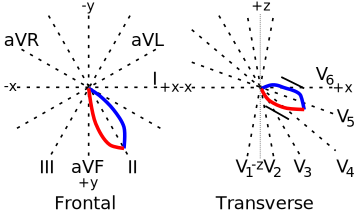
\includegraphics{figures/intro/vector_loops}
\end{center}
\caption[Schematic Vector Loops]{
\label{fig:intro:ecg:planes}
Schematic vector loops showing the relationships of the leads to the frontal and
transverse plane.
The lines of the leads are indicated in heavy-set black lines, the axes in grey
dots when they do not coincide with a lead.
The schematic loops are shown in red and blue, with arrows to indicate the
direction of inscription.
The afferent, or outgoing, limb of the loop is shown in red.
The efferent, or incoming, limb of the loop is shown in blue.
}
\end{figure}

The vectorcardiographic leads can be combined to visualize the electrical
activity of the heart in three planes.
These are the frontal plane, which combines Y and X, the transverse plane, which
combines X and Z, and the sagittal plane, which combines Y and Z.
The frontal plane is the one in which the limb leads measure, whilst the transverse plane
can be related to the precordial leads, as illustrated in
figure~\ref{fig:intro:ecg:planes}.

Dower~\cite{Dower1980}\ proposed a series of coefficients for the three Frank
leads that would convert the Frank leads into the standard 12 lead ECG.
However, the Frank leads are not recorded in common clinical practice.
To remedy this fact, Edenbrandt and Pahlm~\cite{Edenbrandt1988} (and others, for
example~\cite{Uijen1988}), proposed an `inverse dower' transformation.
The inverse dower transform is a set of $8\times3$ coefficients
(table~\ref{tbl:intro:ecg:inverse_dower}) which are used to multiply the eight
independent components of the twelve lead ECG (I, II, $\text{V}_{\text{1--6}}$)
to form the three Frank leads.


\begin{table}
\caption[Inverse Dower Factors after Edenbrandt and Pahlm]{
\label{tbl:intro:ecg:inverse_dower}
Factors to construct the Frank VECG from the standard 12 lead ECG
set~\cite{Edenbrandt1988}.
Each of the 8 leads are multiplied by the given parameters to provide the
orthogonal Frank lead.
}
\begin{center}
\begin{tabular}{c c c c c c c c c}
\toprule
& $\text{V}_{\text{1}}$ &$\text{V}_{\text{2}}$ & $\text{V}_{\text{3}}$ &
$\text{V}_{\text{4}}$ & $\text{V}_{\text{5}}$ & $\text{V}_{\text{6}}$ & I & II \\
\midrule
X & $-0.172$ & $-0.073$ & $0.122$ & $0.231$ & $0.239$ & $0.193$ & $0.156$ & $-0.010$ \\
Y & $0.057$ & $-0.019$ & $-0.106$ & $-0.022$ & $0.040$ & $0.048$ & $-0.227$ & $0.886$ \\
Z & $-0.228$ & $-0.310$ & $-0.245$ & $-0.063$ & $0.054$ & $0.108$ & $0.021$ & $0.102$ \\
\bottomrule
\end{tabular}
\end{center}
\end{table}




\subsection{Body Surface Potential Mapping Arrays}

Body surface potential mapping arrays consist of many electrodes distributed
over the body and recorded simultaneously.
These allow the whole of the body surface potential to be examined and
to be used to establish diagnostic
criteria (for example, \cite{Dubuc1993,SippensGroenewegen1998}).
Mapping systems are also important for so called `inverse solutions', where the
cardiac sources are estimated from the external potentials (for example,
\cite{Ramanathan2006}).
They are also used for the construction of new lead sets (for example,
\cite{Sobieszczanska2007}).
Arrays of anywhere from 16 to over 200 electrodes have been used in such
studies.

\chapter{Applications Of The Forward Problem}

The ECG is the first tool cardiac doctors turn to when diagnosis of a problem is
required.
ECG machines can be found in almost every hospital in the world.
A model of the atria and the surface potentials developed by the excitation of
the model can be used to guide diagnosis of a variety of conditions.
This can reduce the need for surgical procedures or suggest when they are
essential.

Whilst the inverse problem promises to reproduce the potentials on the heart
from the potentials on the surface, the technique has limitations.
For accurate solutions, patient specific geometries have to be constructed from
MRI scans.
There is also a need for complex lead systems, sometimes featuring more than two
hundred leads.
Also, many of the inverse techniques rely on `smooth' propagation patterns to
reduce the uncertainties in the technique which may not be found in pathological
cases.
A device which can perform such calculations automatically is a long way off,
both in terms of computational power required and complexities to resolve.

By contrast, diagnostic guides based on a forward solution can be of use to any
doctor.
They can also be used to further validate simulation studies of genetic or
diseased conditions, by comparison of the generated ECGs with those recorded
from real patients.
This chapter explores some of these predictions, using the model developed in
the previous chapter.

\section{Inverted P-Waves at Night}

Recently an observation was made~\cite{BoyettPrivate}\ concerning patients under
24 hour ECG monitoring.
It was noted that some patients exhibited inverted P-waves at night.
That is to say, if the patient showed a positive P-wave in leads II and aVF
during the day, then at night the P-wave would be negative in leads II and aVF.
These patients had no known heart disease or conduction defects.
This phenomena has not been reported in the literature.

There is evidence~\cite{Shibata2001,Boineau1988,Dobrzynski2005} that the pacemaker is not a
small and discrete area of the atrium, but is instead distributed along the
length of the crista terminalis.
The presence of certain drugs and hormones, most notably acetylcholine, can cause
the site of the leading pacemaker to move down the pace maker complex.
Acetylcholine is released by what is know as increased `vagal tone'.
This has been observed to happen at night.
It was hypothesised that a pacemaker shift induced by this increased vagal tone
might lead to the observed P-wave inversion.

\subsection{Methods}

In the absence of a model for the distributed pacemaker complex in the human
heart, the direct effects of acetylcholine could not be investigated.
Instead, using the model presented in the previous chapter, several sites were
located along the crista terminalis.
These sites had a radius of 15 nodes (or approximately \mm{5}--although this
varied depending on the thickness of the atrial wall at the pacing site), and
therefore were approximately the same size as the sino-atrial node.
These sites are shown in figure~\ref{fig:forward:ct_sites}.
Each of these sites was stimulated via the same protocol used to stimulate the
sinus node in the original model and then the electrical excitation waves were
allowed to propagate without interference.

ECGs were computed from the patterns of electrical excitation in the atrium.
These were compared to the sinus rhythm ECGs computed in the previous chapter.
In addition, using a so called `inverse Dower' method after Edenbrandt and
Pahlm~\cite{Edenbrandt1988}, the orthogonal components of the ECG were computed
and used to construct representations of the heart
vector~\cite{Frank1956,MacFarlane1989a} ECG (VECG).
To perform the inverse dower transformation, a matrix that has been optimized for
the P-wave (shown in Table~\ref{tbl:forward:idparams}) was
used~\cite{Guillem2007}.


\begin{table}
\caption[Inverse Dower Factors]{
\label{tbl:forward:idparams}
Factors to construct the Frank VECG from the standard 12 lead ECG set.
Parameters optimised to accurately reproduce the P-wave heart
vector~\cite{Guillem2007}.
Each of the 8 leads are multiplied by the given parameters to provide the
orthogonal Frank lead.
}
\begin{center}
\begin{tabular}{c c c c c c c c c}
\toprule
& $\text{V}_{\text{1}}$ &$\text{V}_{\text{2}}$ & $\text{V}_{\text{3}}$ &
$\text{V}_{\text{4}}$ & $\text{V}_{\text{5}}$ & $\text{V}_{\text{6}}$ & I & II \\
\midrule
X & $-0.266$ & $\:0.027$ &  $\:0.065$ & $\:0.131$ & $\:0.203$ & $\:0.220$ & $\:0.370$ & $-0.154$ \\
Y & $\:0.088$ &  $-0.088$ & $\:0.003$ & $\:0.042$ & $\:0.047$ & $\:0.067$ & $-0.131$ & $\:0.717$ \\
Z & $-0.319$ & $-0.198$ & $-0.167$ & $-0.099$ & $\:0.009$ & $\:0.060$ & $\:0.184$ & $\:0.114$ \\
\bottomrule
\end{tabular}
\end{center}
\end{table}

\subsection{Results}

\subsubsection{Activation Sequence}

The activation sequences of the atria after pacing from the sinus node, and the
three sites along the crista terminalis are shown in
figure~\ref{fig:forward:inverse:active}\ as isochronal colour maps.
Time goes from red, at \ms{0}, to blue, at \ms{150}.
The site of first activation obviously shifts depending on the stimulus
location.
In addition, as the stimulus site moves away from the sinus node, the time to
total activation of the atria increases.

\begin{figure}
\begin{center}

\includegraphics{figures/forward/inverted_p_wave/activation_sequence}
\end{center}
\caption[Activation sequences from pacing sites along the CT]{
\label{fig:forward:inverse:active}
Atrial activation sequences obtained from different pacing sites.
Shown are the activation sequences resulting from pacing at the sinus node, (s),
and the three crista terminalis sites A--C (a--c).
Activation times are represented by colours, going from red at $\leq$\ms{5}\
through green, \ms{75} to deep blue at \ms{150}.
Contours are every \ms{5}.

There are two views shown for each pacing site.
(i), a view of the right atrial surface with the superior vena cava at the top
of the right atrial surface and the tricuspid valve at the base.
In this view, the crista terminalis runs approximately vertically.
(ii), a view up into the atrial cavities through the valve openings.
The ribbed structures of the pectinate muscles are visible through the tricuspid
valve as they extend off the crista terminalis on the left of the panel.
The right and left atrial appendages are to the top of the panels.

In panel (s) the sinus rhythm activation sequence is visible with rapid
conduction along the crista terminalis and pectinate muscles.
The Bachmann's bundle meanwhile rapidly conducts the excitation to the left
atrium.
In both atria, the appendages are amongst the last regions to depolarise.

In panel (a), the activation sequence has shifted slightly down the crista
terminalis.
The pectinate muscles and crista terminalis still have a large influence on the
propagation.
In both atria, the appendages are the last regions to depolarise.

In panel (b), the activation sequence is shifted a long way down the crista
terminalis.
The Bachmann's bundle is no longer the site of first activation of the left
atrium.
Total time to activate is noticeably delayed.

In panel (c), the activation sequence is shifted a long way down the crista
terminalis.
Total time to activate is noticeably delayed in the left atrium.
The Bachmann's bundle is no longer the site of first activation, instead the
area close to the coronary sinus is first activated.
}
\end{figure}

The sinus node activation sequence,
figure~\ref{fig:forward:inverse:active}(s)(i, ii), starts high on the right
atrium, close to the superior vena cava.
Conduction is especially rapid down the crista terminalis and along the
pectinate muscles, visible as the more widely spaced isochrones along these
structures.
The Bachmann bundle, meanwhile, conducts the electrical excitation to the left
atrium, where it then starts to spread over the left atrial endocardial surface.
In the right atrium the activation finishes, after approximately \ms{80}\ have
elapsed since stimulation started, with the activation of the ring around the
tricuspid valve and the right atrial appendage.
In the left atrium, the far extremities of the left atrial appendage and the far
side of the mitral valve to the Bachmann bundle are activated at approximately
\ms{120}, completing the activation of the atria.

The activation sequence from site A,
figure~\ref{fig:forward:inverse:active}(a)(i, ii), starts high on the right
atrium in the region where the pectinate muscles are branching from the crista
terminalis.
This leads to rapid conduction down the pectinate muscles and in both directions
along the crista terminalis.
The Bachmann bundle conducts the excitation to the left atrium, where it starts
to spread.
The activation of the right atrium finishes with the activation of the right
atrial appendage and then region between the septum and the tricuspid valve.
Activation of the left atrium completes in \ms{132}\ after the initial stimulus
on the edge of the left atrial appendage and the mitral valve.

Pacing from site B leads to the activation sequence depicted in
figure~\ref{fig:forward:inverse:active}(b)(i, ii).
The activation sequence starts lower on the crista terminalis, and is conducted
in both directions along the muscle ridge.
The pectinate muscles also influence the conduction, although the excitation
wavefront reaches them later.
Excitation still reaches the left atrium through the Bachmann bundle, although
it is also conducted through the septum close to the inferior vena cava.
The last point to be excited in the right atrium is still the appendage.
In the left atrium, the last activation comes at \ms{140}.
The left atrial appendage and the sheaths of the pulmonary veins both finish
activating at this time.

The activation sequence which results from pacing from site C is shown in
figure~\ref{fig:forward:inverse:active}(c)(i, ii).
The activation sequence starts low on the right atrium and spreads in all
directions, but is faster travelling up the crista terminalis.
The pectinate muscles, when the excitation wave reaches them, also have a
noticeable effect, speeding activation of the right atrium.
Once again, the left atrium appears to be excited in two places, both by the
bachmann's bundle and close to the inferior vena cava through the septum.
The right atrial appendage is the last region of the right atrium to be excited.
In the left atrium, the extremities of the appendage and the pulmonary vein
sheaths are the last to be excited, as well as the region close to the mitral
valve.
This activation starts at approximately \ms{140}.

All of the activation sequences are approximately normal, in that they travel
from right to left.
The further the stimulus site is removed from the sinus node, the longer
excitation tends to take.


\subsubsection{Twelve Lead ECG}

The ECGs from the three pacing locations along the CT are shown in
figure~\ref{fig:forward:inverse:ecgs}\ with the sinus rhythm P-wave ECG for
comparison.
A summary of the lead deflections for the four cases and sinus rhythm are
presented in table~\ref{tbl:forward:inverse:ecgs}.
There is a clear evolution of the P-wave morphology visible as the pacing site
is moved down the crista terminalis.

\begin{table}
\caption[Lead classification under pacing from different locations]{
\label{tbl:forward:inverse:ecgs}
Lead classification after pacing from different locations.
Leads are classified based on the criteria used by
Kistler~et~al.~\cite{Kistler2006}.
A positive P-wave is denoted by a $+$ sign, a negative P-wave by a $-$ sign and
a biphasic one by $\sim$.
Site denotes the pacing site, where S is the sinus node and Sites A--C are as
indicated in Figure~\ref{fig:forward:ct_sites}.
}
\begin{center}
\begin{tabular}{c c c c c c c c c c c c c}
\toprule
Site & I & II & III & aVR & aVL & aVF & $\text{V}_{\text{1}}$ &$\text{V}_{\text{2}}$ & $\text{V}_{\text{3}}$ & $\text{V}_{\text{4}}$ & $\text{V}_{\text{5}}$ & $\text{V}_{\text{6}}$\\
\midrule
S   & $+$ & $+$ & $\sim$ & $-$ & $+$ & $+$ & $-$ & $+$ & $+$ & $+$ & $+$ & $+$ \\
A   & $+$ & $+$ & $\sim$ & $-$ & $+$ & $\sim$ & $-$ & $+$ & $+$ & $+$ & $+$ & $+$ \\
B   & $+$ & $\sim$ & $-$ & $-$ & $+$ & $-$ & $+$ & $+$ & $+$ & $+$ & $+$ & $+$ \\
C   & $+$ & $-$ & $-$ & $-$ & $+$ & $-$ & $+$ & $+$ & $+$ & $+$ & $+$ & $+$ \\
\bottomrule
\end{tabular}
\end{center}
\end{table}

\begin{figure}
\begin{center}
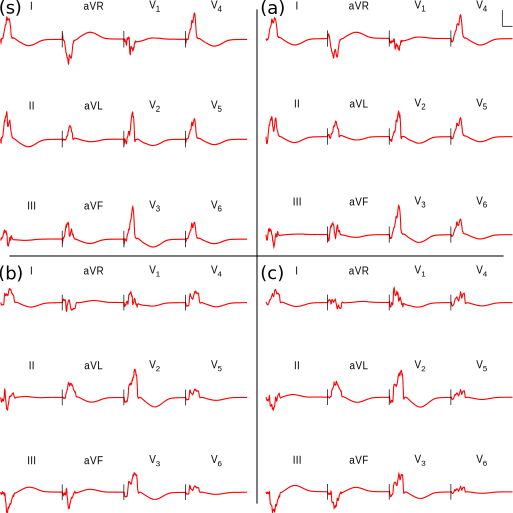
\includegraphics{figures/forward/inverted_p_wave/inverted_pwave_ecg}
\end{center}
\caption[12 Lead ECG traces from pacing sites along the CT]{
\label{fig:forward:inverse:ecgs}
Twelve lead ECG recordings obtained from the model after pacing at the sinus
node, (s) and the three pacing sites A--C (a--c).
Shown is one complete P-wave and $\text{T}_{\text{P}}$ wave, pacing at a rate of
\unit{60}{bpm}.
The scale is the same for all traces, indicated in the top right of panel (a).
The P-wave is positive in leads II and aVR after pacing from the sinus node.
It is positive in leads II and aVR after pacing from site A.
Pacing from site B leads to a negative P-wave in lead aVF and a biphasic P-wave
in lead II.
Site C shows negative P-waves in both leads II and aVR.
}
\end{figure}


The P-wave ECG for pacing from the sinus node,
figure~\ref{fig:forward:inverse:ecgs}(s), is positive in leads II and aVF.
Leads I, aVL and $\text{V}_{\text{2--6}}$ are also positive.
Leads aVR and $\text{V}_{\text{1}}$ are negative.
Lead III is biphasic.
The largest positive lead is $\text{V}_{\text{3}}$, which attains a potential
difference of \mv{+0.390} and the largest negative lead is aVR,
which attains a potential difference of \mv{-0.299}.
The definite positive P-waves in the last 5 precordial leads,
$\text{V}_{\text{2--6}}$, suggest normal propagation through the atrium, with
depolarisation travelling from right to left.
The cardiac axis is approximately $+30^\circ$ in the frontal plane.


Pacing from site A (figure~\ref{fig:forward:inverse:ecgs}(a)), the P-wave ECG is
positive in leads II and  aVF.
Leads I, aVL and $\text{V}_{\text{2--6}}$ are also positive.
Lead aVR and $\text{V}_{\text{1}}$ are negative.
Lead III is biphasic.
The largest positive lead is $\text{V}_{\text{3}}$, which attains a potential
difference of \mv{+0.358} and the largest negative lead is aVR,
which attains a potential difference of \mv{-0.240}.
The definite positive P-waves in the last 5 precordial leads,
$\text{V}_{\text{2--6}}$, suggest normal propagation through the atrium, with
depolarisation travelling from right to left.
The cardiac axis is approximately $+30^\circ$ in the frontal plane.
There is a very prominent notch visible in both leads II and aVF, caused by ...
foo!

Pacing from site B (figure~\ref{fig:forward:inverse:ecgs}(b)), the P-wave ECG is
biphasic in lead II and negative in lead aVF.
Leads I, aVL and $\text{V}_{\text{1--6}}$ are positive.
Lead III and aVR are negative.
The largest positive lead is $\text{V}_{\text{2}}$, which attains a potential
difference of \mv{+0.356} and the largest negative lead is III,
which attains a potential difference of \mv{-0.258}.
The definite positive P-waves in the last 5 precordial leads,
$\text{V}_{\text{2--6}}$, suggest normal propagation through the atrium, with
depolarisation travelling from right to left.
The propagation up the crista terminalis, not down it, is evidenced in the
positive P-wave in $\text{V}_{\text{1}}$.
The cardiac axis is approximately $-30^\circ$ in the frontal plane, due to
activation now travelling up the atrium, rather than down.


Pacing from site C (figure~\ref{fig:forward:inverse:ecgs}(c)), the P-wave ECG is
negative in lead II and lead aVF.
Leads I, aVL and $\text{V}_{\text{1--6}}$ are positive.
In addition to leads II and aVF, lead III and lead aVR are negative.
The largest positive lead is $\text{V}_{\text{2}}$, which attains a potential
difference of \mv{+0.343} and the largest negative lead is III,
which attains a potential difference of \mv{-0.263}.
The positive P-waves in leads $\text{V}_{\text{2--6}}$ suggest that the
propagation is still from right to left, although the low amplitudes in the
later leads suggests that this is not as uniform as in the previous cases.
The propagation up the crista terminalis, not down it, is evidenced in the
positive P-wave in $\text{V}_{\text{1}}$.
The cardiac axis is approximately $-60^\circ$ in the frontal plane, due to
activation now travelling up the atrium, rather than down.

As the pacing site moves down the crista terminalis there is an evolution of the
P-wave, which is visible in all leads.
As a result of the shift, the cardiac axis shifts through about $90^\circ$
anti-clockwise from the sinus direction of $+30^\circ$.
The P-wave duration increases slightly as the crista terminalis increases,
highlighting the importance of the specialized conduction structures of the
heart in rapidly conducting the excitation wave.


\subsubsection{Derived Vector ECGs}

The derived vector ECG plots are shown for the frontal plane in
figure~\ref{fig:forward:inverse:vec_front} and in the transverse plane in
figure~\ref{fig:forward:inverse:vec_trans}.
Again, the sinus rhythm is included in both figures for reference.
The colour of the vector loop represents the passage of time and is coloured
from purple, at \ms{0}, through blue, green, yellow and ending up red at
\ms{500} after initiation of the P-wave.

The vector loop in the frontal plane for sinus rhythm is shown in
figure~\ref{fig:forward:inverse:vec_front}(s).
The vector loop is inscribed in an anti-clockwise direction.
The efferent limb is at approximately \degr{+60}, before it loops up to its
maximal extension at approximately \degr{+45}.
There is a small sub-loop on the afferent limb as the vector trace reaches the
\degr{+30}\ line.
This is possibly caused as the excitation wavefront loops around the tricuspid
valve and the right atrial appendage depolarises.
The $\text{T}_{\text{P}}$ wave is visible as a small anti-clockwise loop,
aligned at approximately \degr{-135}.
The initial deflection along the same line is an artefact of the stimulus
protocol.

The frontal plane vector loop for pacing from site A,
figure~\ref{fig:forward:inverse:vec_front}(a), is inscribed in an anti-clockwise
direction in general.
The main axis of the loop is at approximately \degr{+35}.
The efferent limb is aligned at approximately \degr{+60}, along the line of lead
II.
The afferent limb shows a large loop, which corresponds to the notch in the 12
lead ECG.
The small shift in the pacing site appears to have a relatively large influence
on the 
The $\text{T}_{\text{P}}$ wave is visible as a small loop, aligned at
approximately \degr{-150}.

Pacing from site B produces the frontal plane vector loop in
figure~\ref{fig:forward:inverse:vec_front}(b).
The loop is a figure-of-eight which is initially anti-clockwise.
The main axis of the loop is at approximately \degr{+0}.
The efferent limb is initially aligned at \degr{+30}\ before it sweeps around to
\degr{-60}.
The afferent limb loops back on itself, to \degr{-10} before it returns to the
centre.
The $\text{T}_{\text{P}}$ wave is visible as a small anti-clockwise loop, aligned at
approximately \degr{+150}.
The loop is smaller than that which is observed in the two preceeding pacing
locations.

The frontal plane vector loop from pacing at site C is shown in
figure~\ref{fig:forward:inverse:vec_front}(c).
The loop is open, and inscribed in a clockwise direction.
The main axis of the loop is aligned at approximately \degr{-40}.
The efferent limb oscillates as it travels out along an approximately
\degr{-60}\ vector.
The loop then sweeps down to \degr{-30}, before the afferent limb oscillates as
it returns to 0.
The $\text{T}_{\text{P}}$ is a small clockwise loop at an angle of \degr{+150}.
The loop from site C is the smallest of the loops.

As the pacing site moves down the crista terminalis there are clear changes in
the morphology and principle axis of the P-wave frontal vector loop.
The axis shift which could be determined from the 12 lead ECG was clearly
highlighted.
The vector loops also show the reduction in amplitude of the P-wave as the
pacing location is moved down the crista terminalis, possibly caused by the
generally slower speed of activation.

\subsection{Discussion}

As the stimulus site moves down the crista terminalis the patterns of electrical
activation in the atrium change noticeably.
The focal point of excitation obviously moves down the crista terminalis to
follow this.
It is also interesting to note the similarities.
Despite the shifting activation site, the right atrial appendage and the region
between the tricuspid valve and the atrial septum are always the last to
activate in the right atrium.
In the left atrium, the appendage also activates last in all cases.

As the pacing site moves away from the sinus node, the total activation time
increases.
However, total activation times remain within those observed clinically by
Lemery~et~al.~\cite{Lemery2004}\ for all three pacing locations away from the
sinus node.
The activation patterns are similar to those observed by
Bouineau~et~al.~\cite{Bouineau1988}\ as the pacing location moves, although the
Bouineau data does not include single activations away from the sinus node.

The latter two sites (B \& C), which are low on the crista terminalis, appear to
reach the left atrium in part through a site which emerges close to the coronary
sinus~\cite{Platonov2007,Platonov2008,Markides2003,Lemery2004}.
There is no specialist inferior intra-atrial conduction pathway in the model
however.
Conduction along this lower route is therefore at the normal bulk tissue rate.
It is possible if this were treated specially in the model total activation
times would be reduced.

The ECGs generated from the model also show an evolution as the stimulus site
moves down the crista terminalis.
This change is more visible in the limb leads than in the precordial leads.
This is to be expected, as the propagation remained from right to left in all
cases, but whether it is travelling up or down the atria changes as the pacing
site does.
The P-waves in leads II and aVF is positive in during sinus rhythm, and both
gradually invert as the pacing site shifts down the crista terminalis, as
hypothesised.

As the pacing site moves away from the sinus node, the P-wave duration also
increases.
Especially for the lower crista terminalis sites (B \& C), the duration exceeds
normal P-wave limits~\cite{Lemery2004,Macfarlane1989}.
It is possible that a more detailed intra-atrial conduction system, including an
inferior pathway would reduce total conduction time, and therefore P-wave
duration in these cases.

The P-wave vector loops are similar to those observed in clinical
studies~\cite{Carlson2005,Holmqvist2007,Havmoller2007,Guillem2007}, although the typical
presentation of such loops as monochromatic does make comparison of the timing
information and direction of inscription hard.
They make it quite obvious that the cardiac axis shifts as the pacing location
does.
The morphology of the loops can be used to gain further clues, such as with the
initial rise and then fall visible in the Site B frontal vector loops.

The limitations of the body surface potential model have been discussed
previously (Section X.X.X).
Of particular importance to this study is the lack of a distributed sinus node
model~\cite{Yamamoto2007,Dobrzynski2005}\ for the human atrium.
However, pacemaker shift under the influence of
acetylcholine~\cite{Shibata2001}\ has been observed in rabbits and in
humans~\cite{Opthof1988}\ so it seems plausible as a mechanism for the shifts
and associated P-wave inversions.
The use of an inverse dower matrix to obtain the frank leads rather than
directly measuring them was chosen to allow more direct comparison with clinical
data, which is often only for the standard twelve leads.
The selection of the correct transform matrix is
important~\cite{Guillem2007,Luo1991,Hyttinen1995}\ and it is possible that the
vector loop accuracy could be improved by the use of a transformation matrix
optimised for the body surface potential model.
Alternatively a true frank lead system, or a hybrid model could be constructed.

\subsection{Conclusions of the Inverted P-Wave Study}

The hypothesis that P-wave inversion could be caused by pacemaker shift in the
human sinus node seems to be plausible.
Progressive shift of the pacemaker site down the sinus node leads to progressive
inversion of the observed P-waves in leads II and aVF.
In addition, this shift is accompanied by other changes which do not stray too
far from normality.
This is important, as the shift was originally observed in those with no
diagnosed cardiac disorders.
Further investigation is merited, once an appropriate model of the distributed
sino-atrial node complex can be integrated into the atrial model.

This study shows that the body surface potential model can be used for a study
which involves conditions that begin to deviate from normality.
It can therefore be used as a powerful tool for investigating the clinically
observable consequences of changes to cardiac behaviour.
This can be accomplished without the need for costly clinical trials.



\section{Focal Atrial Tachycardia}

Atrial Tachycardias are one of the rarer forms of supraventricular
tachycardia.
They account for approximately 10\% of diagnosed supraventricular tachycardias/
They tend to occur as a result of other cardiac or respiratory diseases.
They are characterised by a high heart rate ($\leq$ \unit{250}{bpm}) and
typically have evidence of an abnormal cardiac axis or P-wave
morphology~\cite{MacFarlaneSinus1989}.
They are hard to treat with drugs, but radiofrequency ablation can be used with
a high probability of success.
Diagnosis of atrial tachycardia can be difficult due to a lack of data.
Attempts to locate the sites of the ectopic focus are current topics of clinical
research~\cite{Kistler2006,Kahn2006,Yamane2001}.
This study shows how the model can provide more data for clinicians to study.

\subsection{Model of Focal Atrial Tachycardia}

To model focal atrial tachycardia, the model developed in the previous chapter
is used.
Instead of pacing from the cells corresponding to the sinus node, various sites
around the atria are selected.
These sites are shown in figure~\ref{fig:forward:fat:sites}.
Their antatomic locations are summarised in table~\ref{tbl:forward:fat:sites}.
All the nodes which have active cells within 10 cells (\mm{3.3}) are excited via
direct current injection of \unit{2}{nS}\ for \ms{2}.
The resulting excitation wave is then allowed to propagate without interference
and the BSPM, ECG and derived VECG calculated.
The algorithm developed by Kistler~et~al.~\cite{Kistler2006}\ is applied to the
12 lead ECG and the origin of the focal point tachycardia estimated.

\subsection{Results}

\subsubsection{Twelve Lead ECG}

Pacing the atria from different sites results in a dramatic variability in the
observed waveforms of the P-wave ECG.
The ECGs corresponding to the stimuli are shown in
figure~\ref{fig:forward:fat:ecgs}.
The classifications of the waveforms are shown in
table~\ref{tbl:forward:fat:ecgs}.
Classifications consider only the P-wave, and not the $\text{T}_{\text{P}}$
wave.
In the case of more than two significant deflections, the largest two are
chosen.
The effect of any electrical flow is exaggerated by the large P-wave magnitudes
previously noted and so it is likely that with correct magnitudes in the
P-waves, these lesser deflections would not show.


\begin{table}
\caption[Lead classification from pacing sites through the atria]{
\label{tbl:forward:fat:ecgs}
Lead classification after pacing from sites along the crista terminalis.
Leads are classified based on the criteria used by
Kistler~et~al.~\cite{Kistler2006}.
A positive P-wave is denoted by a $+$ sign, a negative P-wave by a $-$ sign and
a isoelectric (no significant positive or negative component) one by $\sim$.
In the case of a biphasic wave, it is classified based on the polarity of the
two component waves, separated by a slash.
Site denotes the pacing site as illustrated in figure~\ref{fig:forward:fat:sites}.
Site S denotes pacing from the sinus node, and is provided for comparison.
}
\begin{center}
\begin{tabular}{c c c c c c c c c c c c c}
\toprule
Site & I & II & III & aVR & aVL & aVF & $\text{V}_{\text{1}}$ &$\text{V}_{\text{2}}$ & $\text{V}_{\text{3}}$ & $\text{V}_{\text{4}}$ & $\text{V}_{\text{5}}$ & $\text{V}_{\text{6}}$\\
\midrule
S & $+$ & $+$ & $+$ & $-$ & $-$ & $+$ & $+/-$ & $+/-$ & $+$ & $+$ & $+$ & $+$ \\
A & $-$ & $+$ & $+$ & $-$ & $-$ & $+$ & $+$ & $+$ & $+$ & $+$ & $+$ & $+$ \\
B & $-$ & $+$ & $+$ & $-$ & $-$ & $+$ & $+$ & $+$ & $+$ & $+$ & $+$ & $+$ \\
C & $\sim$ & $-$ & $\sim$ & $+$ & $\sim$ & $\sim$ & $+$ & $+$ & $+$ & $-$ & $-$ & $-$ \\
D & $+$ & $\sim$ & $-$ & $-$ & $+$ & $-$ & $+$ & $+$ & $+$ & $+$ & $+$ & $+$ \\
E & $+$ & $+$ & $+$ & $-$ & $-$ & $+$ & $-$ & $-$ & $\sim$ & $+$ & $+$ & $+$ \\
F & $+/-$ & $-$ & $-$ & $+$ & $+$ & $-$ & $-/+$ & $-/+$ & $-$ & $-$ & $-$ & $-$ \\
G & $+$ & $-$ & $-$ & $+$ & $+$ & $-$ & $\sim/+$ & $-/+$ & $-$ & $-$ & $-$ & $-$ \\
H & $+$ & $+$ & $-/+$ & $-$ & $+$ & $+$ & $+/-$ & $+/-$ & $+$ & $+$ & $+$ & $+$ \\
\bottomrule
\end{tabular}
\end{center}
\end{table}

Pacing from site A, shown in figure~\ref{fig:forward:fat:ecgs}(a), results in a
P-wave which is positive in most leads.
The P-wave is positive in leads II, III, aVF and $\text{V}_{\text{1--6}}$.
It is negative in leads I, aVR and aVL.
The sharp negative spike visible in $\text{V}_{\text{1}}$ at approximately
\ms{110} is caused by ....
Due to the very short duration of the spike ($\leq$\ms{15}) and the return to
above the baseline, it was discounted from the classification of the wave as
`positive' (Rather than positive/negative biphasic).
Many of the limb leads show a quite ragged profile, and are slightly bifid.

Pacing from site B, shown in figure~\ref{fig:forward:fat:ecgs}(b), results in a
P-wave which is positive in most leads.
The P-wave is positive in leads II, III, aVF and $\text{V}_{\text{1--6}}$.
It is negative in leads I, aVR and aVL.
All of the inferior leads (II, III and aVF) are smooth but highly bifid.
This occurs as the P-wave depolarises first down the left atrium and then the
right, away from the left limb lead electrode.
After the initial depolarisation of the left atrium from the top and right,
towards the left, much of the excitory activity is parallel to the lateral
precordial leads ($\text{V}_{\text{4--6}}$).

Pacing from site C, shown in figure~\ref{fig:forward:fat:ecgs}(c), results in a
P-wave which is relatively flat.
The P-wave is positive in aVR and $\text{V}_{\text{1--3}}$.
It is negative in leads II and $\text{V}_{\text{4--6}}$.
It is biphasic in leads I, III, aVL, aVF.
The signal in all leads, though especially III, aVF and $\text{V}_{\text{4}}$ is
highly variable.
This is due to an uneven propagating wavefront, caused by the anatomical
obstacles.

Pacing from site D, shown in figure~\ref{fig:forward:fat:ecgs}(d), results in a
P-wave which is mostly positive.
The P-wave is positive in leads I, aVL and $\text{V}_{\text{1--6}}$.
It is clearly bifid in all the leads it is positive in, except lead
$\text{V}_{\text{1}}$.
The P-wave is negative in leads III, aVR and aVF.
It is bifid in both III and aVR.
The ECG is biphasic in lead II.

Site E is shown in figure~\ref{fig:forward:fat:ecgs}(e).
The P-wave is positive in lead I, II, III, AVF and $\text{V}_{\text{5, 6}}$.
The P-wave is negative in lead aVR, aVL and $\text{V}_{\text{1--3}}$.
The P-wave is biphasic in lead $\text{V}_{\text{4}}$.
It is bifid in the positive leads II, III and aVF and in the negative leads aVR,
aVL and $\text{V}_{\text{1, 2}}$.
The P-wave is smooth in most leads, aside from the bifidity.
The electrical excitation is spreading down and slightly to the left of the
body, leading to the very positive potentials observed in the inferior leads,
and the positive potentials in leads $\text{V}_{\text{4--6}}$.
The negative potentials in leads $\text{V}_{\text{1, 2}}$ suggest a spread of
excitation anterior to posterior.

Pacing from site F, figure~\ref{fig:forward:fat:ecgs}(f), produces predominately
negative P-waves.
The P-wave is positive in leads aVR and aVL.
It is negative in leads II, III, aVT and $\text{V}_{\text{3--6}}$.
It is biphasic in leads I, $\text{V}_{\text{1}}$ and $\text{V}_{\text{2}}$.
The P-wave is generally quite clean in all the leads, although it shows
significant oscillation at the end of the P-wave in leads II, III and aVF.
This is likely causes as the excitation wave which is spreading up the right
atrium encounters the complex anisotropy of the junctions between the crista
terminalis and the pectinate muscles.


Pacing from site G, shown in figure~\ref{fig:forward:fat:ecgs}(g), produces a
predominately negative P-wave.
The P-wave is positive in leads I, aVR and aVL.
It is negative in leads II, III, aVF and leads $\text{V}_{\text{3--6}}$.
It is biphasic in leads $\text{V}_{\text{1}}$ and $\text{V}_{\text{2}}$.
The negative leads $\text{V}_{\text{3--6}}$ are indicative of a left atrial
pacing site, with the excitation mostly spreading away from the left.
The positive P-wave in leads aVR and aVL, combined with the negative P-waves in
leads II, III and aVF, suggest the excitation is at the base of the heart and is
spreading upwards.
The lead traces are generally clean.

Site H, figure~\ref{fig:forward:fat:ecgs}(h), produces jagged P-waves.
The P-wave is positive in leads I, II, aVL and $\text{V}_{\text{4--6}}$.
The P-wave is negative in lead aVR.
The P-wave is $-/+$ biphasic in leads III, aVF and $\text{V}_{\text{3}}$.
It is $+/-$ biphasic in leads $\text{V}_{\text{1}}$ and $\text{V}_{\text{2}}$.
Leads II, $\text{V}_{\text{4}}$ and $\text{V}_{\text{5}}$ are bifid.
In addition, leads aVF and $\text{V}_{\text{3}}$ are very bifid in appearance,
although the trough becomes negative enough to classify them as biphasic.

\subsubsection{Application of the Focus Location Algorithm}

The algorithm developed by Kistler~et~al. was applied to the P-wave morphologies
generated by the model.
The algorithm is presented as a simple decision tree, initially concerning the
morphology of lead $\text{V}_{\text{1}}$.
The results of applying the algorithm and the actual anatomical locations are
shown in table~\ref{tbl:forward:fat:kistler}.


\begin{table}[h]
\caption[Classification of focal point tachycardia]{
\label{tbl:forward:fat:kistler}
Classification of the origin of focal point tachycardia according to the
algorithm developed by Kistler~et~al. compared with the actual anatomic
location.
Where the algorithm presents multiple sites as a possibility, both are given.
Abbreviations: AA = atrial appended, PV = pulmonary vein, TA = tricuspid anulus,
CS = coronary sinus, S = septum, CT = crista terminalis.
L and R denote left and right, respectively.
}
\begin{center}
\begin{tabular}{l l l}
\toprule
Site & Predicted  & Origin \\
\midrule
A & LAA / LPV & PV \\
B & LAA / LPV & PV \\
C & RPV & PV \\
D & RPV & PV \\
E & RAA / TA & RAA \\
F & CS os / LS & CS \\
G & CS os/ LS & LS \\
H & CT & CT \\
\bottomrule
\end{tabular}
\end{center}
\end{table}

\subsection{Discussion and Conclusions}



\section{Cardiac Simulation Toolkit}

To extract useful results from cardiac modelling two principle components are
needed, as has been previously mentioned: the mathematical models used for
cardiac activity and a computational representation of the experimental
protocols followed to produce results.  A cardiac simulation toolkit provides
one or both of these components to an investigator, removing the need for the
investigator to implement those components themselves.  The word toolkit is
chosen to differentiate from the relatively more common practice of just
providing individual cell models.  A toolkit implies more than one model, or
variants on a model, with a common calling interface and implementation of one
or more experimental protocols or a non-programmatic way of setting up such
protocols---whether through a GUI or through command-line options or
configuration files.

Toolkits have a number of advantages to the investigator, including a reduction
in the work required to bring a paper to publication, increased consistency both
within and outside of the group, fewer implementation mistakes, increased
possibilities for collaboration and verification and a greater accessibility to
cardiac simulations for non-programmers.  The disadvantages of toolkits are not
as numerous, but they too will be considered.  A toolkit will need auditing, to
ensure that the results it gives are accurate.  Toolkits can also constrain the
avenues of experimentation pursued by an investigator by making protocols easier
or harder to implement.  Finally, the additional complexity makes adding any new
feature a little harder---there is a `feature cost'.

\subsection{Advantages of Cardiac Simulation Toolkits}



Cardiac simulation toolkits have existed in one form or another for some
time and include both commercial and open source 
Several cardiac simulation systems have previously been released, one of
the first of which is the OXSOFT HEART~\cite{Noble-1999}.

